\RequirePackage{float}
\documentclass[pdflatex,sn-mathphys-num]{sn-jnl}

% --- Fonts and encodings -------------------------------------------------
% cmap: embeds Unicode ToUnicode CMaps into the PDF so that Cyrillic text
%       can be correctly searched and copy-pasted from the resulting PDF.
% fontenc[T2A]: Cyrillic output encoding used for the Russian text.
% inputenc utf8: declares that source file is UTF-8 encoded.
% type1ec (together with cm-super installed system-wide): forces vector
%       Type 1 outlines for all Computer Modern glyphs, including Cyrillic
%       ones, so the PDF is fully scalable and text extraction works.
\usepackage{cmap}%
\usepackage[T2A]{fontenc}%
\usepackage[utf8]{inputenc}%
\usepackage{type1ec}%
\usepackage[english,russian]{babel}%
\usepackage{graphicx}%
\usepackage{amsmath,amssymb,amsfonts}%
\usepackage{amsthm}%
\usepackage{xcolor}%
\usepackage{booktabs}%
\usepackage{algorithm}%
\usepackage{algorithmicx}%
\usepackage{algpseudocode}%
\usepackage{tabularx}%

\newcommand{\E}{\mathbb{E}}
\newcommand{\I}{\mathbb{I}}

\newtheorem{proposition}{Утверждение}
\newtheorem{definition}{Определение}
\newtheorem{assumption}{Предположение}

\makeatletter
\providecommand*{\toclevel@algorithm}{1}
\providecommand*{\theHalgorithm}{\thealgorithm}
\makeatother

\begin{document}
\selectlanguage{russian}

\title[Hybrid-INoT: гибридная агентная архитектура с внутренней ролевой сегрегацией]{Hybrid-INoT: гибридная агентная архитектура с внутренней ролевой сегрегацией для инженерных задач в условиях длинного общего контекста}

\author*[1]{\fnm{Даниил} \sur{Привезенцев}}\email{daprivezentsev@edu.hse.ru}

\affil*[1]{\orgname{Национальный исследовательский университет <<Высшая школа экономики>>}, \orgaddress{\city{Москва}, \country{Россия}}}

\abstract{Внешняя мультиагентная оркестрация повторно передаёт общий контекст отдельным ролям и увеличивает токенный расход. В работе предложена \textbf{Hybrid-INoT}~--- гибридная система, в которой planner, worker и critic разделяют один вызов модели, а верификация и инструменты остаются внешними. Проверка с сохранёнными артефактами сравнивает полный пакет B3~--- объединённый вызов и детерминированный отбор контекста свыше 4096 токенов~--- с трёхвызовным B2 без компрессии. В реальном API-пилоте Gemini~3.1~Pro Preview ($n=5$ уникальных задач) B3 снизил средний токенный расход на 55.6--88.9\% при целевых контекстах 256--16\,384 токена; независимая репликация Gemini~3.1~Flash-Lite ($n=20$, seed 42) дала 49.6--90.3\%. Средние внутрипарные приросты $U_{\mathrm{tok}}$ Flash-Lite равны 106.5, 144.8, 183.3 и 934.6\%, причём каждая наблюдаемая пара превысила 15\%; условный signed-rank анализ чувствительности прошёл поправку Холма ($p=9.54\cdot10^{-7}$). Четырёхточечные task-level OLS-сводки равны 3.425 для B2 и 0.219 для B3 токена на токен контекста (условный парный $p=1.91\cdot10^{-6}$); это не локальные производные через границу компрессии. Наблюдается эффект системного пакета, а не изолированной оркестрации. Обе архитектуры достигли pass@1${}=1.0$; при нуле вредных исходов среди 20 уникальных пар iid-биномиальная планировочная граница равна 13.91 п.п., поэтому неухудшение в пределах 2 п.п. не доказано. Малая модель идеально согласуется с сохранёнными исходами HumanEval, но плохо~--- с приближённым SWE-bench Lite; эффект политики перезапуска не оценивался. Pro-пилот даёт \$429.96 экономии API-инференса на 10\,000 задач, а task-cluster ресэмплирование~--- диапазон устойчивости \$417.33--\$442.90, но не популяционный интервал и не полный TCO. Данные поддерживают механизм ресурсной эффективности в фиксированных выборках, оставляя открытыми сохранение качества, пользу маршрутизатора, вклад компонентов и перенос на реальные репозитории.}

\keywords{Большие языковые модели, агентные системы, Introspection of Thought, токенная эффективность, экономика инференса, HumanEval, воспроизводимый эксперимент}

\maketitle

\section{Введение}\label{sec:intro}

Современный агент для программной инженерии должен последовательно понять постановку задачи, извлечь релевантный контекст из репозитория и построить изменение, которое затем можно проверить тестами или статическим анализом. На практике эти функции часто распределяются между несколькими ролями, причём под \emph{ролью} понимается отдельный инстанс (экземпляр) большой языковой модели или отдельный ИИ-агент с собственной инструкцией и отдельным обращением к API: одна роль строит план, другая предлагает решение, третья критикует промежуточный результат, четвёртая запускает внешнюю проверку. Таким образом, каждая роль~--- это самостоятельный вызов LLM, а не абстрактная функция внутри одного вызова. Такое разбиение удобно концептуально, но становится затратным, когда все роли вынуждены заново читать один и тот же длинный контекст.

В настоящей работе рассматривается именно этот сценарий: задачи, в которых общими для всех ролей оказываются фрагменты кода, документация, сообщения компилятора и журналы выполнения. Нас интересует не только итоговое качество решения, но и цена выбранной схемы оркестрации в токенах, времени ответа и денежной стоимости вызовов. Поэтому далее статья сопоставляет классическую внешнюю мультиагентную организацию с гибридной схемой, в которой ролевая дискуссия частично переносится внутрь одного вызова модели.

\subsection{Проблема многократной передачи контекста и оценка её значимости}

В агентных системах на основе больших языковых моделей типичной конфигурацией является внешняя мультиагентная оркестрация (Classical-MAS): отдельные процессы или вызовы реализуют роли планировщика, исполнителя, критика и тестировщика~\cite{hong2023metagpt,qian2023chatdev,guo2024survey}. В задачах программной инженерии, где несколько ролей читают одни и те же длинные фрагменты кода, логов и документации, такая схема обладает структурным дефектом: \emph{каждая роль получает копию общего контекста $\mathcal{C}_0$ заново}, а между ролями дополнительно курсируют сообщения координации. Для количественной оценки этого эффекта введём следующие обозначения.

\noindent\textbf{Обозначения к формуле ниже.}
\begin{description}
\item[$\mathcal{A}$] --- множество ролей в схеме Classical-MAS, каждая из которых реализована как отдельный вызов большой языковой модели; $|\mathcal{A}|$~--- число таких ролей (мощность множества).
\item[$\mathcal{C}_0$] --- исходный общий контекст задачи (фрагменты кода, документация, журналы выполнения), одинаковый для всех ролей; $|\mathcal{C}_0|$~--- его длина, измеряемая в токенах модели.
\item[$\bar{h}$] --- средняя длина одного координационного сообщения между ролями, также в токенах.
\item[$D_{\text{ctx}}$] --- суммарный токенный расход на повторную передачу общего контекста всем ролям за одну задачу.
\item[$H_{\text{coord}}$] --- суммарный токенный расход на координационные сообщения, которыми роли обмениваются в процессе решения задачи.
\item[$\Theta(\cdot)$] --- стандартная асимптотическая нотация: запись $f=\Theta(g)$ означает, что $f$ растёт не медленнее и не быстрее $g$ с точностью до постоянных множителей.
\end{description}

\noindent В терминах введённых обозначений токенный бюджет схемы Classical-MAS содержит слагаемое
\begin{equation}
D_{\text{ctx}}=\Theta\bigl(|\mathcal{A}|\cdot|\mathcal{C}_0|\bigr),\qquad
H_{\text{coord}}=O\bigl(|\mathcal{A}|^2\cdot\bar{h}\bigr).
\label{eq:ctx-coord}
\end{equation}

\noindent Смысл формулы~\eqref{eq:ctx-coord} следующий. Первый член описывает линейный рост затрат на контекст, если каждая роль перечитывает $\mathcal{C}_0$. Второй член~--- зависящая от топологии верхняя асимптотическая оценка для случая обмена между всеми парами ролей, а не универсальная квадратичная нижняя граница. Поэтому эмпирическая проверка ниже опирается на непосредственно измеренную повторную передачу входа, а не на предположение о полном графе координации.

В выполненном API-пилоте этот структурный эффект наблюдался непосредственно. При целевом контексте 16\,384 токена Classical-MAS расходовал в среднем 59\,631 токен на задачу, из которых 57\,485 (96.4\%) приходились на вход, тогда как Hybrid-INoT расходовал 6\,608 токенов. Стоимость одного случая составила соответственно \$0.14072 и \$0.02949 при зафиксированных ценах Gemini~3.1~Pro Preview~\cite{openrouterpro2026}. Эти значения относятся к первым пяти задачам HumanEval и не должны переноситься на иной состав задач без повторного измерения.

Таким образом, актуальность проблемы определяется проверяемой величиной: в исследованном длинноконтекстном режиме повторная передача входа дала почти девятикратную разницу в суммарных токенах между B2 и B3. Далее теоретическая модель отделяется от эмпирического свидетельства, а область выводов ограничивается фактически выполненными пилотами.

\subsection{Существующие подходы и их ограничения}

Ближайшее поле шире дихотомии <<саморефлексия против MAS>>: внутримодельное уточнение~\cite{madaan2023selfrefine,shinn2023reflexion}, агенты рассуждение--действие~\cite{yao2022react,yang2024sweagent}, многоперсонное prompting одной LLM~\cite{wang2024spp}, ролевая кооперация через общую доску~\cite{dong2024selfcollaboration}, разреженный внешний дебат~\cite{zeng2025s2mad} и намеренно простой ремонт репозиториев Agentless~\cite{xia2024agentless}. Hybrid-INoT непосредственно развивает INoT~\cite{sun2025inot}. Поэтому заявленная новизна узка: операциональная интеграция внутреннего вызова planner--worker--critic, детерминированного отбора контекста, внешней проверки, маршрутизатора развёртывания и аудитируемого учёта ресурсов. Работа не претендует на изобретение ролевого prompting, самокритики, компрессии или инструментальной проверки по отдельности.

\subsection{Основные результаты и вклад статьи}

В статье получены следующие результаты:
\begin{enumerate}
\item[\textbf{C1.}] Операциональное определение Hybrid-INoT с явной сигнатурой состояний, функцией маршрутизации \texttt{RouteMode} и условием завершения внутреннего ролевого цикла (§\ref{sec:method}).
\item[\textbf{C2.}] Утверждение~\ref{prop:inot-vs-mas}, задающее достаточное балансовое условие преимущества полного пакета Hybrid-INoT по токенам (§\ref{sec:analysis}).
\item[\textbf{C3.}] Неравенство~\eqref{eq:small-model-condition}, задающее условие экономической эффективности малой модели самопроверки (§\ref{sec:analysis}).
\item[\textbf{C4.}] Система метрик токенной эффективности, стоимости и поддерживаемости кода с обоснованной формой агрегации (§\ref{sec:metrics}).
\item[\textbf{C5.}] Эмпирическая проверка с сохранёнными артефактами реальных API-вызовов: масштабирование B2 и B3, абляции, разведочная screening-диагностика и межмодельное сравнение E6 (§\ref{sec:eval}).
\item[\textbf{C6.}] Согласованные с данными вердикты: полная составная H1 не доказана, H2 причинно не оценивалась, H3 не поддержана прямым сравнением (§\ref{sec:eval}).
\end{enumerate}

\noindent Исходный код стенда, конфигурации, сырые результаты и скрипт построения таблиц и графиков опубликованы в отдельном репозитории и зафиксированы по commit hash (§\ref{sec:eval}).

\section{Связанные работы и отличие предлагаемого подхода}\label{sec:related}

\subsection{От chain-of-thought к внутреннему ролевому дебату}

В работе Wei et al.~\cite{wei2022cot} показано, что явная вербализация промежуточных шагов рассуждения может повышать качество решения на задачах, требующих нескольких связанных логических переходов. В данном контексте под промежуточными шагами понимаются текстовые фрагменты, с помощью которых модель раскладывает сложный вывод на последовательность локальных подзадач, а под качеством~--- итоговая успешность решения целевой задачи. Подход Self-Refine~\cite{madaan2023selfrefine} формализует цикл <<генератор--обратная связь--исправление>> внутри одной модели; Reflexion~\cite{shinn2023reflexion} дополняет такую схему механизмом рефлексивной памяти, а ReAct~\cite{yao2022react} связывает внутреннее рассуждение с обращениями к внешним действиям и инструментам. Работа Sun и Zeng~\cite{sun2025inot} описывает Introspection of Thought (INoT) как структурированный внутренний дебат нескольких ролей. В то же время Turpin et al.~\cite{turpin2023unfaithful} показывают, что промежуточный текст цепочки не следует интерпретировать как достоверное описание скрытого вычислительного процесса. Поэтому в настоящей работе интроспекция рассматривается прежде всего как вычислительный механизм отбора кандидатов, критики и селективного перезапуска, а не как буквальное окно в скрытое состояние модели.

\subsection{Мультиагентные системы для программной инженерии}

Weiss \cite{weiss1999} и Wooldridge \cite{wooldridge2009} задают теоретическую рамку MAS. MetaGPT \cite{hong2023metagpt} и ChatDev \cite{qian2023chatdev} переносят её в контекст больших языковых моделей: роли реализуются как отдельные вызовы, каждая получает собственную копию контекста. Обзорные работы указывают на два ключевых ограничения Classical-MAS: распространение ошибки по цепочке и рост стоимости координации \cite{guo2024survey,qian2024scaling}. SWE-bench и SWE-agent \cite{jimenez2023swebench,yang2024sweagent} показывают, что практическая автоматизация задач программной инженерии требует длинного контекста и итеративного редактирования, что ещё сильнее обостряет проблему ретрансмиссии $D_{\text{ctx}}$.

Single-Persona Prompting (SPP) моделирует несколько персон через многотуровое prompting одной LLM~\cite{wang2024spp}; Self-Collaboration Code Generation координирует специализированные роли через общую доску и языкового тестировщика~\cite{dong2024selfcollaboration}; S2-MAD сокращает граф коммуникаций внешнего дебата~\cite{zeng2025s2mad}. Agentless показывает, что компактный конвейер локализации, ремонта и проверки может быть сильной базой без сложного общества агентов~\cite{xia2024agentless}. Эти результаты требуют сравнивать не только названия архитектур, но и топологию вызовов и вклад каждого компонента.

\subsection{Компрессия контекста и внешняя верификация}

LongLLMLingua и LLMLingua-2 \cite{jiang2023longllmlingua,pan2024llmlingua2} демонстрируют, что компрессия промпта сохраняет или улучшает качество на длинном контексте при снижении стоимости. Jia et al.~\cite{jia2026compression} применяют этот подход к коду. Для самопроверки кода недостаточно языковой рефлексии: необходимы внешние наблюдаемые сигналы~--- тесты, статический анализ и сообщения компилятора~\cite{bi2024cocogen,su2025static,sepidband2025complexity}.

\subsection{Сопоставление Hybrid-INoT с предшественниками}\label{subsec:distinction}

Для сопоставления ближайших подходов выделим ролевой механизм, топологию вызовов модели, внешнюю проверку, маршрутизацию и явный учёт ресурсов.

\begin{table}[!htbp]
\caption{Сравнение Hybrid-INoT с близкими архитектурными классами}
\label{tab:distinction}
\centering
\footnotesize
\begingroup
\renewcommand{\arraystretch}{1.25}
\setlength{\tabcolsep}{3pt}
\begin{tabularx}{\textwidth}{@{}>{\raggedright\arraybackslash}p{2.15cm}>{\raggedright\arraybackslash}X>{\raggedright\arraybackslash}X>{\raggedright\arraybackslash}X>{\raggedright\arraybackslash}X@{}}
\toprule
Метод & Роли / вызовы & Внешняя проверка & Маршрутизация & Учёт стоимости \\
\midrule
Self-Refine / Reflexion & Итеративная самокритика; повторные вызовы. & Необязательна. & Фиксированная. & Нет учёта контекстного склона. \\
SPP & Несколько персон одной LLM; много туров. & Не центральна. & Фиксированная. & Сокращение вызовов не является estimand. \\
Self-Collaboration & Роли и общая доска; несколько вызовов. & Языковой тестировщик. & Фиксированная. & Без модели контекстного склона. \\
MetaGPT / ChatDev / S2-MAD & Внешние агенты или разреженный дебат. & Зависит от конвейера. & Фиксированный граф. & Системная цена. \\
Agentless & Заданные стадии; мало вызовов. & Проверка патча. & Фиксированные стадии. & Простота и цена ремонта как baseline. \\
Hybrid-INoT & Planner--worker--critic в одном вызове. & Обязательна после генерации. & Флаги tool/parallel. & Токенный баланс, API-цена, контекстный склон. \\
\botrule
\end{tabularx}
\endgroup
\end{table}

Таблица~\ref{tab:distinction} показывает значительное пересечение на уровне компонентов. Проверяемый вклад настоящей работы~--- интегрированный и инструментированный пакет, а не безусловный приоритет архитектурной идеи.

\section{Формальная постановка задачи}\label{sec:problem}

\subsection{Задача}

Введём базовые множества, используемые в формальной постановке задачи. Их содержательный смысл~--- описать, с какими входными и выходными данными работает агент и в каком пространстве задана его случайность.

\begin{description}
\item[$\mathcal{X}$] --- множество \emph{текстовых спецификаций задач}. Каждый элемент $x\in\mathcal{X}$~--- это строка естественного языка (например, сформулированная пользователем задача или формулировка задачи в HumanEval).
\item[$\mathcal{C}$] --- множество \emph{контекстных артефактов}. Каждый элемент~--- это конечная последовательность текстовых фрагментов: файлов кода, кусков документации, сообщений компилятора, журналов выполнения. Конкретный контекст задачи $\mathcal{C}_0\in\mathcal{C}$~--- это набор именно таких артефактов, имеющих отношение к задаче.
\item[$\mathcal{Y}$] --- множество \emph{кандидатных решений}. Каждый элемент $y\in\mathcal{Y}$~--- это текстовый артефакт, например исходный код функции или патч в формате \texttt{unified diff}, который затем подаётся во внешнюю проверяемую функцию (запуск тестов, статический анализ). Таким образом, $y$~--- не числовой вектор, а именно текст.
\item[$(\Omega,\mathcal{F},\mathbb{P})$] --- \emph{вероятностное пространство}, на котором определены все случайные величины задачи. Здесь $\Omega$~--- множество возможных исходов одного запуска агента (все возможные сценарии развития процесса решения), $\mathcal{F}$~--- $\sigma$-алгебра наблюдаемых событий над $\Omega$ (формальная структура, позволяющая корректно говорить о вероятностях событий), $\mathbb{P}$~--- вероятностная мера на $\mathcal{F}$, учитывающая сразу три источника случайности: стохастическую генерацию токенов в LLM при температуре $>0$, выбор начального числа генератора псевдослучайных чисел (\emph{seed}~--- целое число, инициализирующее детерминированную последовательность псевдослучайных чисел; фиксация seed обеспечивает воспроизводимость запуска) и недетерминизм внешних инструментальных вызовов (например, таймауты тестов). Проще говоря, $(\Omega,\mathcal{F},\mathbb{P})$~--- это математический способ записать утверждение <<запуск агента~--- это случайный эксперимент>>.
\end{description}

\begin{definition}[Агентная инженерная задача]\label{def:task}
Агентная инженерная задача~--- это кортеж $(x,\mathcal{C}_0,\mathcal{Z},\mathcal{V})$, где $x\in\mathcal{X}$~--- текстовое описание задания; $\mathcal{C}_0\in\mathcal{C}$~--- исходный контекст задачи, включающий код, документацию и журналы выполнения; $\mathcal{Z}$~--- конечное множество разрешённых внешних инструментов (запуск тестов, линтер, компилятор, поиск по репозиторию и~т.\,п.); $\mathcal{V}\colon\mathcal{Y}\to\{0,1\}$~--- внешняя проверяемая функция успеха, возвращающая~$1$ при корректном решении (например, при прохождении всего тестового набора) и~$0$ иначе.
\end{definition}

\paragraph*{Случайные величины, индуцируемые стратегией агента.} Стратегия агента~--- это зафиксированная процедура, отображающая описание задачи $x$ и контекст $\mathcal{C}_0$ в распределение на $\mathcal{Y}$. Она индуцирует следующие случайные величины (функции из $\Omega$ в числовые множества):
\begin{description}
\item[$Y\colon\Omega\to\mathcal{Y}$] --- \emph{случайный выход агента}: итоговое кандидатное решение, которое агент возвращает в конце работы на конкретном запуске.
\item[$T\colon\Omega\to\mathbb{R}_{\ge 0}$] --- \emph{суммарный токенный расход} на одну задачу. Значение $T(\omega)$~--- общее число токенов (суммарно по всем вызовам модели во всех ролях и итерациях), израсходованных на решение задачи в конкретном запуске $\omega$. Здесь $\mathbb{R}_{\ge 0}$~--- множество неотрицательных действительных чисел.
\item[$C_{\text{inf}}\colon\Omega\to\mathbb{R}_{\ge 0}$] --- \emph{денежная стоимость инференса} на одну задачу (в валюте расчёта, например в долларах США), вычисляемая как произведение числа входных и выходных токенов на соответствующие тарифы API.
\item[$\ell\colon\Omega\to\mathbb{R}_{\ge 0}$] --- \emph{задержка выполнения} одной задачи (wall-clock time в секундах) от получения запроса до возврата решения.
\end{description}
Случайность этих величин обусловлена стохастической генерацией LLM и недетерминизмом внешних инструментов; математическое ожидание $\E[\cdot]$ во всех последующих выражениях берётся по мере $\mathbb{P}$ на $(\Omega,\mathcal{F})$.

\paragraph*{Целевая функция и ограничения.} Цель агента~--- максимизировать ожидаемое качество решения, удерживая ожидаемые затраты в пределах заданных бюджетов. Формально:
\begin{equation}
\max\;\E\bigl[\mathcal{V}(Y)\bigr]\quad\text{при условиях}\quad\E[T]\le B,\;\;\E[C_{\text{inf}}]\le B_{\$},\;\;\E[\ell]\le B_{\ell}.
\label{eq:agent-goal}
\end{equation}

\noindent\textbf{Расшифровка всех величин в~\eqref{eq:agent-goal}:}
\begin{description}
\item[{$\E[\mathcal{V}(Y)]$}] --- математическое ожидание функции успеха $\mathcal{V}$ от случайного выхода~$Y$. Поскольку $\mathcal{V}\in\{0,1\}$, эта величина равна вероятности того, что агент на случайном запуске вернёт корректное решение (то есть $\Pr[\mathcal{V}(Y)=1]$).
\item[{$\E[T]$}] --- среднее число токенов, расходуемых агентом на одну задачу (по распределению, заданному~$\mathbb{P}$).
\item[{$\E[C_{\text{inf}}]$}] --- средняя денежная стоимость инференса на одну задачу.
\item[{$\E[\ell]$}] --- средняя задержка ответа на одну задачу.
\item[{$B,B_{\$},B_{\ell}$}] --- \emph{верхние бюджетные лимиты}, заданные пользователем или эксплуатационным контекстом: $B$~--- допустимый средний токенный расход (в токенах), $B_{\$}$~--- допустимая средняя стоимость (в валюте расчёта), $B_{\ell}$~--- допустимая средняя задержка (в секундах).
\end{description}
\noindent Словами: формула~\eqref{eq:agent-goal} означает <<среди стратегий, укладывающихся в заданные бюджеты по токенам, деньгам и времени, выбрать ту, у которой наибольшая ожидаемая доля успешных решений>>.

\subsubsection*{Сводка обозначений}

Ниже собраны все обозначения, используемые в дальнейшем тексте, с явными определениями. Часть из них введена выше при постановке задачи; остальные появятся в разделах об архитектуре и аналитической модели.

\begin{description}
\item[{$\mathcal{C}_0\in\mathcal{C}$}] --- исходный общий контекст задачи (конечная последовательность текстовых артефактов); $|\mathcal{C}_0|\in\mathbb{N}$~--- его длина в токенах модели.
\item[{$\hat{\mathcal{C}}$}] --- сжатая версия исходного контекста, используемая во внутреннем цикле Hybrid-INoT; $|\hat{\mathcal{C}}|\le|\mathcal{C}_0|$.
\item[{$\mathcal{A}$}] --- конечное множество внешних ролей в схеме Classical-MAS, каждая из которых~--- отдельный вызов LLM; $|\mathcal{A}|\in\mathbb{N}$~--- число таких ролей.
\item[{$Y\colon\Omega\to\mathcal{Y}$}] --- случайный выход агента; $y\in\mathcal{Y}$~--- конкретный (реализованный) кандидат решения.
\item[{$K\in\mathbb{N}$}] --- число кандидатов, одновременно порождаемых ролью $r_{\text{work}}$ на одной итерации внутреннего цикла (базовая конфигурация: $K=3$).
\item[{$T\colon\Omega\to\mathbb{R}_{\ge 0}$}] --- случайная величина суммарного токенного расхода на одну задачу; $\E[T]=\int_{\Omega}T(\omega)\,\mathrm{d}\mathbb{P}(\omega)$~--- её математическое ожидание, вычисляемое по мере $\mathbb{P}$ на вероятностном пространстве $(\Omega,\mathcal{F},\mathbb{P})$, введённом выше.
\item[{$U_{\text{tok}}=Q/T$}] --- показатель токенной эффективности: отношение агрегированной оценки качества $Q$ (см.~§\ref{sec:metrics}) к суммарному токенному расходу; единица измерения~--- <<качество на 1000~токенов>>.
\item[{$\tau^\star\in\mathbb{R}_{\ge 0}$}] --- теоретическая точка пересечения, следующая только из достаточных балансовых предположений; эксперимент E3 её не идентифицирует.
\item[{$\delta_{H1}\in(0,1)$}] --- минимальный практически значимый относительный прирост показателя $U_{\text{tok}}$, используемый в гипотезе H1 (базовое значение $\delta_{H1}=0{,}15$, то есть 15\%).
\item[{$C_{\text{check}}^S\in\mathbb{R}_{\ge 0}$}] --- денежная стоимость одной предварительной проверки решения, выполняемой \emph{малой} (дешёвой) моделью самопроверки; верхний индекс $S$ обозначает small.
\item[{$C_{\text{rerun}}^L\in\mathbb{R}_{\ge 0}$}] --- денежная стоимость одного повторного запуска \emph{крупной} (дорогой) модели; верхний индекс $L$ обозначает large.
\item[{$\rho_0,\rho_1\in[0,1]$}] --- вероятности того, что потребуется дорогостоящий повторный запуск крупной модели: $\rho_0$~--- без предварительной проверки малой моделью, $\rho_1$~--- при наличии такой проверки; по построению $\rho_1\le\rho_0$.
\item[{$\E[\cdot]$}] --- математическое ожидание на вероятностном пространстве $(\Omega,\mathcal{F},\mathbb{P})$.
\item[{$\mathbb{I}[\,\cdot\,]$}] --- индикаторная функция: $\mathbb{I}[\text{A}]=1$, если условие A истинно, и $0$ иначе.
\end{description}

\subsection{Гипотезы исследования}

Перед формулировкой гипотез поясним несколько обозначений и статистических процедур, встречающихся ниже, чтобы избавить читателя от необходимости искать их на стороне.

\begin{description}
\item[<<п.п.>> (процентные пункты)] --- единица разности двух величин, выраженных в процентах. Если одна конфигурация даёт pass@1 $=68\%$, а другая $=66\%$, то разница составляет $2$~процентных пункта ($68-66=2$), но при этом относительное изменение равно $\approx 3\%$. В тексте всегда используется <<п.п.>> именно в этом смысле: абсолютная разность процентов, а не отношение.
\item[Парный критерий Вилкоксона (Wilcoxon signed-rank test)] --- непараметрический статистический тест для сравнения двух связанных выборок (например, значений метрики на одних и тех же задачах при двух конфигурациях). В отличие от $t$-критерия не требует нормальности распределения; проверяет гипотезу о симметрии распределения разностей относительно нуля. Применяется стандартно при небольших и негауссовских выборках~\cite{wilcoxon1945}.
\item[Поправка Холма--Бонферрони (Holm--Bonferroni correction)] --- пошаговая процедура корректировки уровня значимости при множественном сравнении. Если одновременно проверяется $m$ гипотез с $p$-значениями $p_{(1)}\le p_{(2)}\le\dots\le p_{(m)}$, то $k$-я гипотеза отвергается, если $p_{(k)}\le\alpha/(m-k+1)$. Эта поправка контролирует вероятность хотя бы одной ложной находки (family-wise error rate) при $\alpha=0{,}05$ и является менее консервативной, чем обычная поправка Бонферрони~\cite{holm1979}.
\item[task-resampling диапазон устойчивости] --- квантили $2{,}5\%$ и $97{,}5\%$ статистики после $10^4$ ресэмплирований наблюдаемых задач с возвращением. Для первых неслучайно выбранных задач этот диапазон показывает чувствительность к их перевзвешиванию, но не является design-based доверительным интервалом для популяции.
\item[seed (начальное число генератора псевдослучайных чисел)] --- целое число, которым инициализируется локальная псевдослучайная последовательность и передаётся поддерживающему этот параметр API. Фиксация seed обеспечивает повторяемость локальной выборки, но сама по себе не гарантирует битовую воспроизводимость закрытой LLM.
\item[Synthetic Tool-Use Suite] --- контролируемый микротест стенда для сравнения последовательного и параллельного выполнения независимых инструментальных задержек. Он не является внешним бенчмарком и используется только как проверка механизма H3; точная реализация находится в сопроводительном репозитории.
\end{description}

\begin{description}
\item[\textbf{H1} (преимущество при длинном контексте).] Существует пороговая длина исходного контекста $\tau^\star$ такая, что при $|\mathcal{C}_0|>\tau^\star$ архитектура Hybrid-INoT обеспечивает рост показателя $U_{\text{tok}}$ не менее чем на $\delta_{H1}=15\%$ по сравнению с Classical-MAS, при этом качество решения (pass@1) не ухудшается более чем на $2$~п.п.\par\emph{Проверка:} E3 (§\ref{subsec:e3}) сообщает среднее по конечному набору и число пар выше порога; критерий Вилкоксона, task-resampling диапазоны и поправка Холма являются условным анализом чувствительности, а не design-based выводом о популяции.
\item[\textbf{H2} (экономическая оправданность малой модели самопроверки).] Существует режим, в котором предварительная проверка малой моделью уменьшает вероятность дорогостоящего повторного запуска настолько, что выполняется условие~\eqref{eq:small-model-condition}: $C_{\text{check}}^S<(\rho_0-\rho_1)\,C_{\text{rerun}}^L$.\par\emph{Предусмотренная проверка:} интегрированный policy-эксперимент с per-case решениями о перезапуске и затратами. Сохранённый E4 (§\ref{subsec:e4}) этому дизайну не соответствует и используется только как разведочная диагностика screening.
\item[\textbf{H3} (граница применимости).] При задачах с истинно независимыми подзадачами и параллельными инструментами преимущество Hybrid-INoT по времени ответа исчезает или становится отрицательным.\par\emph{Проверка:} архитектурное сравнение на пяти задачах и отдельный контролируемый микротест последовательных/параллельных инструментов E2c (§\ref{subsec:e2}).
\end{description}

В H1 внутри пары фиксированы модель, инструменты, верификация, задача, seed, температура и промпт задачи. Однако treatment является \emph{системным пакетом}: B2 использует три вызова над несжатым контекстом, а B3 объединяет ролевые префиксы в одном вызове и применяет детерминированный отбор свыше 4096 токенов. Поэтому E3 оценивает эффект пакета, а не изолированный причинный вклад оркестрации или компрессии. Порог $\delta_{H1}=15\%$~--- минимально практически значимый эффект; экономия ресурсов не подменяет полный составной критерий H1.

\section{Метод: Hybrid-INoT}\label{sec:method}

\subsection{Определение метода и базовая идея}\label{subsec:method-intro}

Прежде чем переходить к формальному описанию, дадим содержательное определение метода, на котором строится предлагаемая архитектура, и сформулируем саму идею Hybrid-INoT в минимально необходимой форме.

\begin{definition}[Introspection of Thought, INoT]\label{def:inot}
\emph{Introspection of Thought} (INoT)~--- это приём организации рассуждений большой языковой модели, при котором \emph{внутри одного обращения} к модели разворачивается структурированный диалог нескольких \emph{ролей} (ролевых префиксов: <<планировщик>>, <<исполнитель>>, <<критик>> и~т.\,п.). Каждая роль читает и дописывает общий рабочий буфер в рамках одного прогона модели, что позволяет удерживать общий контекст без дублирования~\cite{sun2025inot}. В отличие от внешней мультиагентной оркестрации, каждая роль INoT \emph{не} является отдельным вызовом LLM~--- это ролевой префикс внутри единственного вызова.
\end{definition}

\begin{definition}[Hybrid-INoT]\label{def:hybrid-inot}
\emph{Hybrid-INoT}~--- архитектура, предлагаемая в настоящей работе, которая комбинирует внутренний ролевой цикл \emph{planner--worker--critic} в смысле Определения~\ref{def:inot} с \emph{обязательной} внешней инструментальной проверкой и предобработкой контекста. А именно:
\begin{itemize}
\item роли планирования ($r_{\text{plan}}$), генерации кандидатов ($r_{\text{work}}$) и критики ($r_{\text{crit}}$) выполняются как ролевые префиксы внутри одного вызова крупной LLM над сжатым общим контекстом $\hat{\mathcal{C}}$;
\item вовне вынесены три и только три класса операций: (i)~компрессия контекста $\mathcal{C}_0\mapsto\hat{\mathcal{C}}$ (отдельным лёгким модулем), (ii)~внешняя проверяемая верификация $r_{\text{self}}$ (запуск тестов, статического анализа, компилятора), (iii)~функция маршрутизации \texttt{RouteMode}, решающая, какой режим работы применить к данной задаче.
\end{itemize}
Таким образом, Hybrid-INoT~--- это промежуточная конфигурация между чисто внутриконтекстной самокритикой (Self-Refine, Reflexion) и полностью внешней мультиагентной оркестрацией (MetaGPT, ChatDev), у которой \emph{внутри} сохраняется разделяемый контекст и ролевая сегрегация, а \emph{снаружи} остаются только операции с проверяемыми, инструментальными сигналами.
\end{definition}

Дальнейшие подпункты формализуют эту идею: §\ref{subsec:states-sigs}~--- состояния и сигнатуры ролей, §\ref{subsec:routemode}~--- функция маршрутизации, §\ref{subsec:inner-loop}~--- внутренний цикл и условие его завершения, §\ref{subsec:compression}~--- компрессия контекста, §\ref{subsec:selective-rerun}~--- селективный перезапуск.

\subsection{Состояния и сигнатуры ролей}\label{subsec:states-sigs}

Определим состояние системы $\sigma=(x,\hat{\mathcal{C}},\mathcal{H},i)$, где $x\in\mathcal{X}$~--- текстовое описание задачи (см.~Определение~\ref{def:task}), $\hat{\mathcal{C}}$~--- сжатый общий контекст, $\mathcal{H}$~--- история итераций, $i\in\{0,\dots,I\}$~--- счётчик итераций, а $I\in\mathbb{N}$~--- верхний предел числа итераций. Отдельно общий API-клиент ведёт денежный счётчик эксперимента и отклоняет запрос, если его оценочная стоимость пересечёт настроенный жёсткий лимит.

Пусть $\Pi$~--- \emph{пространство планов}, то есть множество возможных текстовых планов решения (в базовой реализации~--- короткий маркированный список шагов на естественном языке). Пусть $K\in\mathbb{N}$~--- \emph{число кандидатных решений, одновременно порождаемых ролью $r_{\text{work}}$ на одной итерации внутреннего цикла}; в базовой конфигурации $K=3$. Тогда каждая роль задаётся сигнатурой $r\colon\mathcal{S}_r^{\text{in}}\to\mathcal{S}_r^{\text{out}}$:
\begin{align}
r_{\text{plan}} &\colon(x,\hat{\mathcal{C}})\mapsto \pi\in\Pi, \label{eq:sig-plan}\\
r_{\text{work}} &\colon(\pi,\hat{\mathcal{C}},K)\mapsto \mathbf{y}=(y_1,\dots,y_K)\in\mathcal{Y}^K, \label{eq:sig-work}\\
r_{\text{crit}} &\colon(\mathbf{y},\hat{\mathcal{C}})\mapsto (s_1,\dots,s_K)\in[0,1]^K, \label{eq:sig-crit}\\
r_{\text{self}} &\colon(y\in\mathcal{Y})\mapsto (v,M,e)\in\{0,1\}\times[0,1]\times\mathcal{E}. \label{eq:sig-self}
\end{align}

\noindent\textbf{Расшифровка сигнатур~\eqref{eq:sig-plan}--\eqref{eq:sig-self}:}
\begin{description}
\item[$r_{\text{plan}}$] --- роль \emph{планировщика}. Входы: текст задачи $x$ и сжатый контекст $\hat{\mathcal{C}}$. Выход: план $\pi\in\Pi$~--- последовательность шагов решения.
\item[$r_{\text{work}}$] --- роль \emph{исполнителя} (генератора кандидатов). Входы: план $\pi$, сжатый контекст $\hat{\mathcal{C}}$, число требуемых кандидатов $K$. Выход: набор $\mathbf{y}=(y_1,\dots,y_K)$ из $K$ кандидатных решений $y_k\in\mathcal{Y}$; запись $\mathcal{Y}^K$~--- $K$-я декартова степень множества~$\mathcal{Y}$. Значение $K$ задаётся гиперпараметром архитектуры (в базовой конфигурации $K=3$) и регулирует разнообразие: при $K=1$ критик всегда оценивает единственный вариант и роль $r_{\text{crit}}$ вырождается; увеличение $K$ повышает вероятность получить хоть одно корректное решение ценой пропорционального роста выходных токенов.
\item[$r_{\text{crit}}$] --- роль \emph{критика}. Входы: набор кандидатов $\mathbf{y}$ и контекст $\hat{\mathcal{C}}$. Выход: набор скалярных оценок $(s_1,\dots,s_K)\in[0,1]^K$, где $s_k$~--- оценка качества $k$-го кандидата (1~--- безусловно принять, 0~--- безусловно отвергнуть).
\item[$r_{\text{self}}$] --- \emph{внешний процесс самопроверки}: запуск тестов, статического анализа и линтера. Вход: один отобранный кандидат $y$. Выход: тройка $(v,M,e)$, где $v\in\{0,1\}$~--- бинарный вердикт, $M\in[0,1]$~--- оценка поддерживаемости (см.~формулу~\eqref{eq:maintainability}), а $e\in\mathcal{E}$~--- подтверждённое инструментами сообщение об ошибке.
\end{description}

\noindent Роли $r_{\text{plan}},r_{\text{work}},r_{\text{crit}}$ реализуются как ролевые префиксы внутри \emph{одного} вызова крупной модели над общим $\hat{\mathcal{C}}$; роль $r_{\text{self}}$~--- отдельный внешний процесс (запуск тестов, линтера, статического анализатора). Содержательный смысл сигнатур: внутренний цикл вырабатывает план, по нему генерирует $K$ кандидатов, оценивает их критиком и передаёт лучшего на внешнюю инструментальную проверку, которая возвращает единственный объективный сигнал об успехе.

\subsection{Функция маршрутизации}\label{subsec:routemode}

\paragraph*{Содержательный смысл.} \texttt{RouteMode} выбирает внутренний либо внешний рабочий процесс по двум дешёвым признакам задачи: обязательности внешнего инструментального workflow и доминирующему параллелизму подзадач. Ниже приведено правило, реально присутствующее в зафиксированном commit.

\begin{definition}[RouteMode]\label{def:routemode}
Пусть $\varphi_{\mathrm{tool}}(x)\in\{0,1\}$ считывает Boolean-поле metadata \texttt{requires\_tool}, а $\varphi_{\mathrm{par}}(x)\in\{0,1\}$ равно единице, когда поле metadata \texttt{parallelism} не меньше двух. Тогда
\[
\texttt{RouteMode}(x)=\begin{cases}\texttt{external}, & \varphi_{\mathrm{tool}}(x)=1 \;\lor\; \varphi_{\mathrm{par}}(x)=1,\\ \texttt{internal}, & \text{иначе}.\end{cases}
\]
Зафиксированный код не выводит эти флаги из произвольной инструкции: для синтетических tool-задач их задаёт загрузчик benchmark. Обучаемый или инструкционный metadata-классификатор и порог по длине контекста возможны как будущие расширения, но в исследуемом commit их нет. В E3 внутренний режим B3 принудительно используется во всех ячейках, поэтому качество маршрутизатора и любой порог маршрутизации не оцениваются.
\end{definition}

\subsection{Внутренний цикл и условие завершения}\label{subsec:inner-loop}

\begin{algorithm}[htbp]
\caption{Hybrid-INoT: внутренний интроспективный цикл}\label{alg:main}
\begin{algorithmic}[1]
\Require задача $x$, контекст $\mathcal{C}_0$, максимум итераций $I$, число кандидатов $K$, лимит перезапусков $R$
\Ensure решение $y^\star$, флаг $v^\star$, оценка $M^\star$
\State $\mathcal{C}\gets\texttt{PolicySanitize}(x,\mathcal{C}_0)$
\State $\hat{\mathcal{C}}\gets\texttt{CompressIfNeeded}(\mathcal{C})$ \Comment{Алг.~\ref{alg:compression}}
\State $m\gets\texttt{RouteMode}(x)$ \Comment{Опр.~\ref{def:routemode}}
\If{$m=\texttt{external}$} \Return \texttt{ExternalAgentWorkflow}$(x,\hat{\mathcal{C}})$ \EndIf
\State $s^{\text{best}}\gets-\infty;\; s^{\text{prev}}\gets-\infty;\; y^{\text{best}}\gets\bot;\; r\gets0;\; e\gets\varnothing$
\For{$i=1$ to $I$}
 \State $(\pi_i,\{y_{i,k}\},\{s_{i,k}\})\gets\texttt{CombinedLargeModelCall}(x,\hat{\mathcal{C}},K,e)$
 \Comment{один API-вызов с ролевыми префиксами}
 \State $k^\star\gets\arg\max_k s_{i,k};\; y_i\gets y_{i,k^\star}$
 \If{$s_{i,k^\star}>s^{\text{best}}$} $s^{\text{best}}\gets s_{i,k^\star};\; y^{\text{best}}\gets y_i$ \EndIf
 \State $(v_i,M_i,e_i)\gets r_{\text{self}}(y_i)$ \Comment{$e_i$: подтверждённый вывод инструментов}
 \If{$v_i=1$} \Return $(y_i,1,M_i)$ \EndIf
 \State $e\gets\texttt{Truncate}(e_i,600)$
 \If{$r<R$}
   \State $(y'_i,v'_i,M'_i,e'_i)\gets\texttt{SelectiveRerun}(x,\{y_{i,k}\},\{s_{i,k}\})$; $r\gets r+1$
   \If{$v'_i=1$} \Return $(y'_i,1,M'_i)$ \EndIf
 \EndIf
 \If{$i>1\land s_{i,k^\star}-s^{\text{prev}}<\varepsilon$} \textbf{break} \Comment{см.~Утв.~\ref{prop:convergence}}\EndIf
 \State $s^{\text{prev}}\gets s_{i,k^\star}$
\EndFor
\State \Return $(y^{\text{best}},0,M(y^{\text{best}}))$
\end{algorithmic}
\end{algorithm}

\begin{proposition}[Терминация внутреннего цикла]\label{prop:convergence}
Пусть каждая операция внутри одной итерации алгоритма~\ref{alg:main} завершается за конечное время, а число итераций ограничено сверху параметром $I$. Тогда алгоритм завершится не позднее чем после $I$ итераций: он либо вернёт решение после успешной внешней проверки, либо после итерации $i>1$ остановится при $s_{i,k^\star}-s^{\text{prev}}<\varepsilon$, либо после исчерпания лимита итераций вернёт лучший найденный кандидат.
\end{proposition}

\begin{proof}
Внешний цикл по индексу $i$ содержит не более $I$ проходов. Каждая итерация включает конечный набор шагов: построение плана, генерацию $K$ кандидатов, критическую оценку, внешнюю проверку и обновление контекста. По предположению все эти операции завершаются за конечное время, следовательно, завершается и любая отдельная итерация. Поэтому алгоритм либо прекращается досрочно по инструкции \textbf{return} или \textbf{break}, либо после $I$-й итерации достигает последней инструкции \textbf{return}. Тем самым время работы внутреннего цикла сверху ограничено конечным числом итераций, а утверждение доказано.
\end{proof}

\subsubsection*{Замечание}
Утверждение~\ref{prop:convergence} гарантирует только завершение алгоритма, но не монотонный рост оценок $s_i$ и не корректность самого критика. Сценарий, в котором критик систематически подтверждает неверные решения, рассматривается отдельно в E2b (§\ref{subsec:e2}) как одна из угроз валидности.

\subsection{Компрессия контекста}\label{subsec:compression}

\begin{algorithm}[htbp]
\caption{Компрессия длинного контекста}\label{alg:compression}
\begin{algorithmic}[1]
\Require $\mathcal{C}_0$, порог длины $\tau_{\text{len}}$
\Ensure $\hat{\mathcal{C}}$
\If{$|\mathcal{C}_0|\le\tau_{\text{len}}$} \Return $\mathcal{C}_0$ \EndIf
\State разбить $\mathcal{C}_0$ на текстовые блоки $\{b_j\}$ и выделить идентификаторы задачи
\State $\text{rel}(b_j)\gets 5\,r_{\mathrm{id}}(b_j)+2\,\mathbb{I}_{\mathrm{sig}}(b_j)+4\,\mathbb{I}_{\mathrm{err}}(b_j)-0.001\,|b_j|$
\State сохранить блоки сигнатур/ошибок; остальные добавлять по убыванию $\text{rel}(b_j)$
\State \Return блоки, сумма proxy-счётчиков которых не превышает $\tau_{\text{len}}=4096$
\end{algorithmic}
\end{algorithm}

Здесь $r_{\mathrm{id}}$~--- доля идентификаторов задачи в блоке, а $\mathbb{I}_{\mathrm{sig}}$ и $\mathbb{I}_{\mathrm{err}}$ отмечают сигнатуры и тексты ошибок/логов. Реализация ограничивает сумму proxy-счётчиков блоков, но затем соединяет их разделителями; поэтому сериализованный контекст может немного превысить 4096 proxy-токенов (наблюдаемый максимум E3~--- 4170). Этот детерминированный лексический proxy вдохновлён обучаемой компрессией~\cite{jiang2023longllmlingua,pan2024llmlingua2}, но не является классификатором LLMLingua-2. Явная формула и описание граничного поведения исключают приписывание эффекта модели, которая фактически не запускалась.

\subsection{Селективный перезапуск}\label{subsec:selective-rerun}

\paragraph*{Содержательный смысл.} \emph{Селективный перезапуск}~--- механизм экономии токенов и денежного бюджета при неудачной попытке решения. Вместо того чтобы при отказе критика перезапускать всю итерацию с нуля или вообще прекращать работу, процедура отбирает $M\le K$ лучших по оценке критика кандидатов, поочерёдно прогоняет их через внешнюю верификацию $\texttt{ExternalVerify}$ и, если ни один не прошёл, формирует новый промпт \emph{только} на основе \emph{подтверждённых} инструментами сигналов ошибки (сообщений тестов, трасс исключений, вывода статического анализатора), а не субъективных комментариев критика. Это ограничивает распространение языковых галлюцинаций между итерациями и уменьшает число дорогих повторных запусков. Алгоритм~\ref{alg:rerun} формализует процедуру.

\begin{algorithm}[!htbp]
\caption{Селективный перезапуск по подтверждённым сигналам}\label{alg:rerun}
\begin{algorithmic}[1]
\Require задача $x$, кандидаты $\{y_1,\dots,y_K\}$, оценки $\{s_k\}$
\Ensure $(y^\star,v^\star,M^\star,e^\star)$
\State отсортировать $\{y_k\}$ по убыванию $s_k$; оставить верхние $M\le K$
\For{каждый $y_m$ из отобранных}
  \State $(v_m,M_m,e_m)\gets r_{\text{self}}(y_m)$
  \If{$v_m=1$} \Return $(y_m,1,M_m,e_m)$ \EndIf
\EndFor
\State сформировать один корректирующий промпт из $x$, лучшего кандидата и $\texttt{Truncate}(e_m,600)$
\State $y'\gets\texttt{LargeModelRerun}(\text{промпт})$
\State $(v',M',e')\gets r_{\text{self}}(y')$
\State \Return $(y',v',M',e')$
\end{algorithmic}
\end{algorithm}

\paragraph*{Расшифровка входов и выходов Алгоритма~\ref{alg:rerun}.}
\begin{description}
\item[$\{y_1,\dots,y_K\}\subset\mathcal{Y}$] --- набор кандидатных решений, полученных от роли $r_{\text{work}}$ на текущей итерации.
\item[{$\{s_1,\dots,s_K\}\subset[0,1]$}] --- соответствующие оценки от роли-критика $r_{\text{crit}}$.
\item[$M\in\{1,\dots,K\}$] --- число кандидатов, допускаемых к \emph{дорогой} внешней проверке (в базовой конфигурации $M=\min(K,3)$).
\item[$\texttt{ExternalVerify}(y_m)\in\{0,1\}$] --- внешняя проверка (вызов тестового раннера, линтера, статического анализатора); возвращает $1$ только при полном успехе.
\item[$(y^\star,v^\star,M^\star,e^\star)$] --- исправленное решение и результат его внешней проверки; общий лимит $R$ проверяется вызывающим Алгоритмом~\ref{alg:main}.
\end{description}

\paragraph*{Почему именно подтверждённые сигналы.} Восстанавливая промпт только из объективных сообщений инструментов, алгоритм обрывает обратную связь <<критик подтверждает собственную ошибку $\to$ следующее поколение наследует её>>, которая систематически ухудшает сходимость в чисто языковых Self-Refine/Reflexion-циклах~\cite{shinn2023reflexion,madaan2023selfrefine}.

\section{Аналитическая модель токенных и стоимостных затрат}\label{sec:analysis}

\subsection{Структура аналитических соотношений}

Анализ в данном разделе включает два типа соотношений. К первому относятся прямые балансовые равенства и неравенства, задающие структуру токенных и денежных затрат. Ко второму относятся утверждения о сравнении архитектур при фиксированных предположениях относительно длины контекста, стоимости координации и внутренней критики. Такое разделение позволяет отличить общие расчётные соотношения от результатов, требующих дополнительных условий.

\subsection{Токенные бюджеты Classical-MAS и Hybrid-INoT}

Перед формулировкой утверждения о преимуществе по токенам введём обозначения для \emph{всех} слагаемых, из которых складываются бюджеты $T_{\text{MAS}}$ и $T_{\text{INoT}}$, и зафиксируем соответствующие предположения. Все величины далее выражены в токенах модели и относятся к одной задаче.

\begin{description}
\item[$T_{\text{MAS}}$] --- суммарный токенный расход агента Classical-MAS на одну задачу (случайная величина по распределению~$\mathbb{P}$).
\item[$T_{\text{INoT}}$] --- суммарный токенный расход агента Hybrid-INoT на одну задачу.
\item[$T_{\text{ctx}}^{\text{MAS}}$] --- вклад повторной передачи общего контекста в бюджет Classical-MAS.
\item[$T_{\text{coord}}^{\text{MAS}}$] --- вклад координационных сообщений между ролями в бюджет Classical-MAS.
\item[$T_{\text{gen}}$] --- совокупный вклад собственно генерации кандидатов и прочих членов, не зависящих линейно от числа внешних ролей $|\mathcal{A}|$ (одинаково присутствующий в обеих архитектурах и потому сокращающийся при вычитании).
\item[$T_{\text{cmp}}$] --- стоимость однократной компрессии контекста $\mathcal{C}_0\mapsto\hat{\mathcal{C}}$.
\item[$T_{\text{core}}^{\text{add}}$] --- дополнительная стоимость внутренней критики в Hybrid-INoT сверх обычной генерации (расход на ролевые префиксы и развёрнутый внутренний дебат).
\item[$T_{\text{check}}$] --- суммарная стоимость внешних верификаций (запусков тестов/линтера, передачи их вывода обратно в модель) за одну задачу.
\item[$T_{\text{rerun}}$] --- случайная величина стоимости повторных запусков при провале внешней верификации.
\item[{$\alpha\in(0,1]$}] --- доля ролей Classical-MAS, читающих полный контекст (см.~Предположение~\ref{as:ctx}).
\item[$\gamma\ge0$] --- коэффициент, ограничивающий стоимость компрессии: $T_{\text{cmp}}\le\gamma|\mathcal{C}_0|$.
\item[$\beta\ge0$] --- коэффициент, ограничивающий дополнительную стоимость критики: $T_{\text{core}}^{\text{add}}\le\beta|\hat{\mathcal{C}}|$.
\item[$I\in\mathbb{N}$] --- верхний предел числа итераций в обеих архитектурах.
\item[$\bar{h}$] --- средняя длина координационного сообщения между ролями (в токенах).
\end{description}

Неотрицательность $\beta$ и $\gamma$ сама по себе не гарантирует преимуществ одной архитектуры. Точное достаточное условие $A_0>0$ ниже совместно зависит от $I$, $\alpha|\mathcal{A}|$, $q_{\max}$, $\beta$ и $\gamma$; его предпосылки подлежат эмпирической проверке для конкретной реализации.

\begin{assumption}\label{as:ctx}
На каждой из $I$ итераций Classical-MAS не менее $\alpha|\mathcal{A}|$ ролей, $\alpha\in(0,1]$, читают общий контекст $\mathcal{C}_0$ целиком. Hybrid-INoT использует выбранный контекст $\hat{\mathcal{C}}$, для которого $|\hat{\mathcal{C}}|\le q_{\max}|\mathcal{C}_0|$ при фиксированном $q_{\max}\le1$.
\end{assumption}

\begin{assumption}\label{as:bounded}
Стоимость однократной компрессии ограничена как $T_{\text{cmp}}\le\gamma|\mathcal{C}_0|$, дополнительная стоимость внутренних ролей~--- как $T_{\text{core}}^{\text{add}}\le\beta|\hat{\mathcal{C}}|$, а модуль разности всех остальных слагаемых генерации, верификации и повторных запусков двух систем не превышает константы $K_0$, не зависящей от $|\mathcal{C}_0|$.
\end{assumption}

\begin{proposition}[Достаточное балансовое условие]\label{prop:inot-vs-mas}
Пусть
\[
A_0=I\alpha|\mathcal{A}|-(I+\beta)q_{\max}-\gamma.
\]
При Предположениях~\ref{as:ctx}--\ref{as:bounded}, если $A_0>0$, то
\begin{equation}
\E[T_{\text{MAS}}-T_{\text{INoT}}]\ge A_0|\mathcal{C}_0|-K_0,
\label{eq:token-advantage}
\end{equation}
и ожидаемая разность токенных расходов положительна при $|\mathcal{C}_0|>K_0/A_0$.
\end{proposition}

\begin{proof}[Балансовый вывод]
Из Предположения~\ref{as:ctx}
\[
T_{\text{ctx}}^{\text{MAS}}\ge I\alpha|\mathcal{A}|\cdot|\mathcal{C}_0|.
\]
Для Hybrid-INoT сумма повторной передачи выбранного контекста, дополнительного расхода внутренних ролей и компрессии ограничена:
\[
(I+\beta)|\hat{\mathcal{C}}|+\gamma|\mathcal{C}_0|
\le\bigl((I+\beta)q_{\max}+\gamma\bigr)|\mathcal{C}_0|.
\]
После вычитания и применения границы $K_0$ ко всем остаточным различиям получаем~\eqref{eq:token-advantage}. При $A_0>0$ её правая часть положительна ровно при $|\mathcal{C}_0|>K_0/A_0$.
\end{proof}

\paragraph*{Область применимости утверждения.} Утверждение~\ref{prop:inot-vs-mas}~--- достаточный балансовый результат для полного системного пакета, а не причинная теорема об одной оркестрации и не валидация маршрутизатора. Неотрицательные координационные расходы Classical-MAS могут усилить границу, но не используются как недоказанная асимптотическая нижняя оценка. E3 оценивает склоны пакетов B2/B3; поскольку пересечение не заключено внутри сетки, эксперимент не идентифицирует ни $K_0/A_0$, ни deployment-порог.

\subsection{Тождество числа запросов и граница выходных токенов}

Реализация получает все $K$ кандидатов, план и критику одним основным вызовом на итерацию; поэтому умножение одного prompt на $K$ дважды учитывало бы общий контекст. Пусть $N_{\mathrm{core}}\le I$ и $N_{\mathrm{rerun}}\le\min(I,R)$~--- фактическое число основных и повторных вызовов, а $P$ и $O$~--- записанные провайдером входные и выходные токены одного вызова. Для внутреннего маршрута выполняется тождество
\begin{equation}
T_{\mathrm{INoT}}^{\mathrm{internal}}
=\sum_{i=1}^{N_{\mathrm{core}}}\bigl(P_{\mathrm{core},i}+O_{\mathrm{core},i}\bigr)
+\sum_{j=1}^{N_{\mathrm{rerun}}}\bigl(P_{\mathrm{rerun},j}+O_{\mathrm{rerun},j}\bigr).
\label{eq:request-accounting}
\end{equation}
В зафиксированной реализации серверные лимиты выхода равны $O_{\mathrm{core},i}\le2048+700K$ и $O_{\mathrm{rerun},j}\le1024$, откуда
\[
T_{\mathrm{out}}\le N_{\mathrm{core}}(2048+700K)+1024N_{\mathrm{rerun}}.
\]
Компрессия детерминирована и не вызывает модель. Бюджет суммы блоков равен 4096 proxy-токенам, но разделители не входят в этот счётчик, поэтому сериализованный контекст E3 достигает 4170 proxy-токенов. Жёсткой границы полного входа нет: постановка задачи не ограничена, а proxy-счётчик может отличаться от токенизации провайдера. Код применяет предзапросный денежный cap в общем API-клиенте, но не per-task token counter. Поэтому мы сообщаем тождество записанного расхода и output-only границу, но не заявляем жёсткую гарантию полного токенного бюджета.

\subsection{Условие экономической эффективности малой модели самопроверки}

\paragraph*{Обозначения для формулы стоимости инференса.} Пусть агент в процессе решения одной задачи делает несколько вызовов крупной (large, верхний индекс $L$) и малой (small, верхний индекс $S$) моделей с индексом $i$, пробегающим по вызовам. Для каждого вызова обозначим:
\begin{description}
\item[$p_i^L,\,r_i^L$] --- число входных (prompt) и выходных (response) токенов $i$-го вызова крупной модели.
\item[$p_i^S,\,r_i^S$] --- то же для $i$-го вызова малой модели.
\item[$c_L^{\mathrm{in}},\,c_L^{\mathrm{out}}$] --- цены \emph{крупной} модели за один входной и выходной токен соответственно (в валюте расчёта, обычно долл. США за токен; у провайдеров API обычно указывается цена за $10^6$ токенов, и значения пересчитываются делением на $10^6$).
\item[$c_S^{\mathrm{in}},\,c_S^{\mathrm{out}}$] --- то же для малой модели.
\end{description}

\begin{equation}
C_{\text{inf}}=c_L^{\mathrm{in}}\sum_i p_i^L+c_L^{\mathrm{out}}\sum_i r_i^L+c_S^{\mathrm{in}}\sum_i p_i^S+c_S^{\mathrm{out}}\sum_i r_i^S.
\label{eq:cost-inference}
\end{equation}

\noindent Формула~\eqref{eq:cost-inference}~--- прямая балансовая запись: денежная стоимость инференса на одну задачу равна сумме по всем вызовам произведений числа токенов на соответствующий тариф, раздельно для входных/выходных токенов и крупной/малой моделей.

\paragraph*{Обозначения для условия эффективности.} Рассмотрим схему, в которой после получения кандидата $y$ крупной моделью он предварительно проверяется \emph{малой} моделью; если малая модель сигнализирует об ошибке, запускается повторная генерация крупной моделью. Введём:
\begin{description}
\item[$C_{\text{check}}^S$] --- денежная стоимость одной предварительной проверки малой моделью (включает входной и выходной токенный расход проверочного вызова, пересчитанный в деньги по~\eqref{eq:cost-inference}).
\item[$C_{\text{rerun}}^L$] --- денежная стоимость одного повторного запуска крупной модели (при провале текущего кандидата).
\item[$\rho_0$] --- вероятность того, что потребуется дорогостоящий повторный запуск \emph{в базовой схеме без малой модели самопроверки} (то есть доля ошибочных кандидатов, не выловленных ни одним дешёвым механизмом).
\item[$\rho_1$] --- та же вероятность \emph{при наличии} предварительной проверки малой моделью; по построению $0\le\rho_1\le\rho_0\le 1$, причём часть ошибочных кандидатов малая модель отсекает, прежде чем они попадут в крупную.
\end{description}

\paragraph*{Вывод условия.} Сравним ожидаемые расходы на одну задачу в двух сценариях.

\emph{Сценарий~0} (без малой модели): расход $=0$ при успехе; с вероятностью $\rho_0$ возникает повторный запуск крупной модели стоимостью $C_{\text{rerun}}^L$. Ожидаемые дополнительные расходы: $\E_0=\rho_0\cdot C_{\text{rerun}}^L$.

\emph{Сценарий~1} (с малой моделью): \emph{всегда} платим $C_{\text{check}}^S$ за предварительную проверку; дополнительно с вероятностью $\rho_1$ всё ещё нужен повторный запуск стоимостью $C_{\text{rerun}}^L$. Ожидаемые дополнительные расходы: $\E_1=C_{\text{check}}^S+\rho_1\cdot C_{\text{rerun}}^L$.

В этой двухсценарной модели с ровно одной предварительной проверкой, не более чем одним предотвращённым перезапуском и постоянной стоимостью перезапуска малая модель экономически эффективна тогда и только тогда, когда $\E_1<\E_0$, то есть
\begin{equation}
C_{\text{check}}^S+\rho_1\cdot C_{\text{rerun}}^L\;<\;\rho_0\cdot C_{\text{rerun}}^L,
\end{equation}
что после переноса $\rho_1\cdot C_{\text{rerun}}^L$ в правую часть даёт
\begin{equation}
C_{\text{check}}^S<(\rho_0-\rho_1)\cdot C_{\text{rerun}}^L.
\label{eq:small-model-condition}
\end{equation}

\noindent\textbf{Содержательная расшифровка~\eqref{eq:small-model-condition}.} Левая часть~--- фиксированная стоимость предварительной проверки. Правая часть~--- ожидаемая экономия \emph{при условии, что интегрированная политика действительно предотвращает часть запусков крупной модели}. Поэтому неравенство является перспективным условием проектирования. Сохранённый E4 содержит только агрегированное согласие screening-процедуры и не реализует и не идентифицирует эффект политики $\rho_0-\rho_1$.

\section{Система метрик}\label{sec:metrics}

\subsection{Основные метрики и обоснование формы агрегации}

Основными количественными характеристиками работы агента в настоящем исследовании выступают токенная эффективность $U_{\text{tok}}$, денежная эффективность $Q_{\$}$ и доля полностью проверенных решений $\mathrm{VCR}$ (Verified Candidate Rate). Приведём сначала определения, затем~--- расшифровку всех входящих величин.

\begin{align}
U_{\text{tok}}&=\frac{Q}{T}, \label{eq:u-tok}\\
Q_{\$}&=\frac{Q}{C_{\text{inf}}}, \label{eq:q-dollar}\\
\mathrm{VCR}&=\frac{1}{N}\sum_{i=1}^{N}\mathbb{I}\bigl[\text{tests}_i=1\;\land\;\text{static}_i=1\;\land\;\text{sec}_i=1\bigr]. \label{eq:vcr}
\end{align}

\noindent\textbf{Расшифровка~\eqref{eq:u-tok}--\eqref{eq:vcr}.}
\begin{description}
\item[$Q$] --- агрегированная скалярная оценка качества решения задачи, принимающая значения на $[0,1]$. По построению $Q$ совпадает с ожидаемым значением функции успеха $\E[\mathcal{V}(Y)]$ (см.~\eqref{eq:agent-goal}), а в случае неоднородного датасета~--- с взвешенной суммой по классам задач $Q=\sum_{b}w_{b}Q_{b}$, где $Q_b\in[0,1]$~--- средняя успешность по классу $b$ (например, <<короткие задачи HumanEval>>, <<длинный контекст SWE-bench>>), а $w_b\ge 0$~--- доля класса в оцениваемой выборке при $\sum_{b}w_{b}=1$.
\item[$T$] --- средний токенный расход на одну задачу (в токенах); $U_{\text{tok}}=Q/T$~--- <<качество, получаемое с 1000 токенов>>, то есть показатель токенной эффективности.
\item[$C_{\text{inf}}$] --- средняя денежная стоимость инференса на одну задачу (см.~\eqref{eq:cost-inference}); $Q_{\$}=Q/C_{\text{inf}}$~--- <<качество, получаемое на 1 доллар>>, то есть показатель денежной эффективности.
\item[$N$] --- число задач в оцениваемой выборке.
\item[$\text{tests}_i\in\{0,1\}$] --- результат прогона автоматического тестового набора по $i$-й задаче: $1$, если \emph{все} тесты пройдены, $0$ иначе.
\item[$\text{static}_i\in\{0,1\}$] --- результат статического анализа (линтера/типизатора): $1$, если не сообщено ни одной ошибки из набора критических правил, $0$ иначе.
\item[$\text{sec}_i\in\{0,1\}$] --- результат проверки безопасности (например, Bandit~/~Semgrep для Python, CodeQL для общих целей): $1$, если не обнаружено ни одной уязвимости, $0$ иначе.
\item[{$\mathbb{I}[\,\cdot\,]$}] --- индикаторная функция: равна $1$, если указанное в скобках условие истинно, и $0$ иначе. В частности, $\mathbb{I}[\text{static}_i=1]$ принимает значение $1$, если статический анализатор для $i$-й задачи не выявил критических замечаний, и $0$ в противном случае.
\item[$\land$] --- логическая конъюнкция (<<и>>): выражение $\text{tests}_i=1\land\text{static}_i=1\land\text{sec}_i=1$ истинно лишь тогда, когда \emph{одновременно} выполнены все три условия.
\end{description}

\noindent\textbf{Содержательный смысл VCR.} Формула~\eqref{eq:vcr} считает \emph{долю} задач, на которых выход агента одновременно прошёл все три класса объективных проверок~--- функциональные тесты, статический анализ и проверку безопасности. Решение засчитывается только при успехе по всем трём критериям: индикатор в сумме даёт $1$, если и только если все три условия истинны, и $0$ иначе. Множитель $\tfrac{1}{N}$ нормирует сумму на число задач~$N$, переводя её в долю от $0$ до $1$ (в процентах~--- от $0\%$ до $100\%$). Таким образом, запись $\tfrac{1}{N}\sum_{i}\mathbb{I}[\dots]$~--- это обычная \emph{средняя доля успехов}, а не произвольный коэффициент $1/3$: тройки условий здесь нет, есть $N$ задач и усреднение по ним.

\paragraph*{Почему именно три критерия.} Три компонента индикатора~--- тесты, статический анализ и проверка безопасности~--- задают \emph{минимально достаточный} набор объективных сигналов для патча в инженерной постановке. Функциональные тесты фиксируют корректность, статический анализ~--- отсутствие явных ошибок и нарушений стиля, проверка безопасности~--- отсутствие уязвимостей. Конъюнкция консервативна: частичный успех (например, <<тесты пройдены, но есть уязвимость>>) не засчитывается, что соответствует практикам промышленного CI/CD.

\subsection{Агрегированная метрика успешности и её форма}

Для агрегированной оценки успешности используется форма
\begin{equation}
\mathrm{MAS}_i=\min(\mathrm{Success}_i,\mathrm{Verified}_i)\cdot M_i^{\lambda},\qquad \lambda\in[0,1],\quad\lambda=0.5.
\label{eq:mas}
\end{equation}
Обоснование этой конструкции состоит в следующем. Во-первых, величины $\mathrm{Success}$ и $\mathrm{Verified}$ являются необходимыми условиями засчитывания решения: patch, не прошедший внешнюю проверку, не должен получать высокий итоговый балл. Во-вторых, множитель $M_i^\lambda$ моделирует влияние поддерживаемости на итоговую оценку; параметр $\lambda$ регулирует силу этого влияния. В базовой конфигурации используется $\lambda=0.5$; анализ E2d обнаружил семь инверсий ранжирования при изменении $\lambda$ и весов, поэтому составная метрика рассматривается только как вспомогательная.

\subsection{Веса поддерживаемости и их обоснование}

\begin{equation}
M_i=w_{\mathrm{cc}}(1-\widehat{\mathrm{CC}}_i)+w_{\mathrm{dup}}(1-\widehat{\mathrm{Dup}}_i)+w_{\mathrm{warn}}(1-\widehat{\mathrm{Warn}}_i)+w_{\mathrm{doc}}\widehat{\mathrm{Doc}}_i.
\label{eq:maintainability}
\end{equation}

\begin{table}[htbp]
\caption{Веса поддерживаемости и их связь с подкатегориями ISO/IEC~25010:2023~\cite{iso25010}}
\label{tab:weights}
\centering
\footnotesize
\begin{tabularx}{\textwidth}{@{}lc>{\raggedright\arraybackslash}X@{}}
\toprule
Параметр & Значение & Обоснование \\
\midrule
$w_{\mathrm{cc}}$ & $0.35$ & ISO 25010 Modifiability; цикломатическая сложность~\cite{mccabe1976}~--- наиболее прямой прокси стоимости сопровождения. \\
$w_{\mathrm{dup}}$ & $0.25$ & ISO 25010 Reusability; дублирование~--- ключевой сигнал технического долга. \\
$w_{\mathrm{warn}}$ & $0.20$ & ISO 25010 Analysability; warnings~--- поверхностный, но надёжный сигнал. \\
$w_{\mathrm{doc}}$ & $0.20$ & ISO 25010 Modifiability; покрытие документацией как прокси понятности. \\
\botrule
\end{tabularx}
\end{table}

\subsubsection*{Анализ чувствительности}
В E2d проверяется устойчивость ранжирования конфигураций B0--B3 при вариации $(w_{\mathrm{cc}},w_{\mathrm{dup}},w_{\mathrm{warn}},w_{\mathrm{doc}})$ в $\pm 20\%$ и при $\lambda\in\{0,0.25,0.5,0.75,1\}$ в~\eqref{eq:mas}. Инверсия ранжирования при таких вариациях рассматривается как признак чувствительности метрики к выбранной параметризации.

\subsection{Метрики надёжности}
\begin{align}
\mathrm{SCR}&=\frac{\#\{\text{ошибочные кандидаты, выявленные процедурой самопроверки}\}}{\#\{\text{все ошибочные кандидаты}\}},\\
\mathrm{RFR}&=\frac{\#\{\text{патчи без отката}\}}{\#\{\text{применённые патчи}\}}.
\end{align}

\section{Эмпирическая валидация}\label{sec:eval}

\subsection{Воспроизводимость, исходные данные и статистический протокол}\label{subsec:e1}

Исследовательский стенд опубликован в репозитории INoT\_Research~\cite{inotresearch2026}; все результаты привязаны к commit \texttt{010211ee5775185e8330ab6cde06e912c2adcb9e}. Проверка \texttt{python -m inot check} завершилась без ошибок, а \texttt{pytest} дал 15 успешных тестов. Исходные JSON находятся в \texttt{results/slide\_e2e3\_real}, \texttt{results/e6} и \texttt{reproducibility/results/20260726\_flash\_lite}; переносимые относительные пути, SHA-256, агрегаты и код рисунков сохранены в \texttt{reproducibility/evidence\_snapshot.json}. Проверка сетки нашла 60/60 ожидаемых строк Pro и 240/240 строк Flash-Lite без дубликатов ключей, пропущенных ячеек, расхождений токенного баланса и usage trace. Единица анализа~--- задача $\times$ архитектура $\times$ целевой контекст $\times$ seed.

Основной набор данных~--- канонический HumanEval~\cite{chen2021humaneval}. Pro-пилот использует задачи HumanEval/0--4, а повторный Flash-Lite-прогон~--- HumanEval/0--19 в исходном порядке. Исторический контекст строится детерминированно (seed 42) из постановок и эталонных решений \emph{других} задач HumanEval; эталон целевой задачи не добавляется. Блоки присоединяются целиком, поэтому фактическая длина может превышать целевую. Для $n=20$ при целевых $\{256,1024,4096,16384\}$ фактические средние длины равны соответственно $\{371.2,1154.8,4210.6,16524.3\}$ токена, а диапазоны~--- $\{259$--$545,\ 1024$--$1411,\ 4100$--$4415,\ 16389$--$16946\}$. Такой контекст воспроизводим, но синтетичен и не моделирует историю реального репозитория во всей полноте.

Сравниваются B2 Classical-MAS (planner, worker и critic как отдельные API-вызовы над несжатым контекстом) и B3 Hybrid-INoT (объединённые ролевые инструкции и детерминированный отбор контекста свыше 4096 токенов). После генерации выполняется внешняя проверка. Следовательно, основной estimand~--- end-to-end контраст пакетов, а не изолированный эффект оркестрации. E3 всегда запускает B3 во внутреннем режиме и не проверяет \texttt{RouteMode}. Pro-пилот выполнен через \texttt{google/gemini-3.1-pro-preview}, репликация~--- через \texttt{google/gemini-3.1-flash-lite}. Цены \$2/\$12 и \$0.25/\$1.50 за миллион входных/выходных токенов зафиксированы 26 июля 2026~г.~\cite{openrouterpro2026,openrouterflash2026}. API-псевдонимы не являются неизменными снимками весов.

Для каждой длины контекста образуется пара B2--B3 на одной задаче и одном seed. Используются
\begin{align}
S_T &= 100\left(1-\frac{\overline{T}_{B3}}{\overline{T}_{B2}}\right), &
S_C &= 100\left(1-\frac{\overline{C}_{B3}}{\overline{C}_{B2}}\right), \label{eq:empirical-savings}\\
\Delta U_{\mathrm{tok}} &= 100\left(\frac{U_{\mathrm{tok}}^{B3}}{U_{\mathrm{tok}}^{B2}}-1\right). \label{eq:empirical-utok}
\end{align}
Средние, минимумы и число пар выше порога рассматриваются как описательные estimand конечного набора. Критерий Вилкоксона~\cite{wilcoxon1945} сообщается только как условный анализ симметричного сдвига распределения и не тестирует приведённое среднее. Для 15\%-го подкритерия односторонний signed-rank тест применяется к $\Delta U_{\mathrm{tok}}-15\%$, а семья четырёх контекстов корректируется процедурой Холма~\cite{holm1979}. Диапазоны по $10^4$ task-level ресэмплированиям показывают устойчивость к перевзвешиванию наблюдаемых задач, но не популяционное покрытие. Для качества рассчитывается вредная дискордантность; нулевая Clopper--Pearson граница служит iid-биномиальным планировочным ориентиром, а не design-valid выводом для первых неслучайных задач HumanEval. Четыре повторных контекста не считаются независимыми исходами, а один сохранённый API-прогон не оценивает вариативность seed или повторных вызовов провайдера.

\subsection{E3~--- Масштабирование по длине контекста}\label{subsec:e3}

Таблица~\ref{tab:e3-results} содержит непосредственно наблюдаемые средние. В обоих прогонах расход B2 растёт почти линейно с добавляемым контекстом, тогда как B3 после 4096 целевых токенов остаётся около 5.6--6.7 тыс. токенов вследствие компрессии.

\begin{table}[htbp]
\caption{Реальные API-измерения B2 и B3 на HumanEval}
\label{tab:e3-results}
\centering
\footnotesize
\begin{tabular}{@{}llrrrrc@{}}
\toprule
Модель & Контекст & $T_{B2}$ & $T_{B3}$ & $S_T$, \% & $S_C$, \% & pass@1 B2/B3 \\
\midrule
Pro ($n=5$) & 256 & 4964 & 2203 & 55.6 & 43.1 & 1.00/1.00 \\
 & 1024 & 7117 & 2925 & 58.9 & 46.8 & 1.00/1.00 \\
 & 4096 & 18218 & 6706 & 63.2 & 49.1 & 1.00/1.00 \\
 & 16384 & 59631 & 6608 & 88.9 & 79.0 & 1.00/1.00 \\
\midrule
Flash-Lite ($n=20$) & 256 & 2738 & 1379 & 49.6 & 26.0 & 1.00/1.00 \\
 & 1024 & 5487 & 2271 & 58.6 & 41.8 & 1.00/1.00 \\
 & 4096 & 16007 & 5664 & 64.6 & 56.9 & 1.00/1.00 \\
 & 16384 & 58110 & 5633 & 90.3 & 86.9 & 1.00/1.00 \\
\botrule
\end{tabular}
\end{table}

\begin{figure}[htbp]
\centering
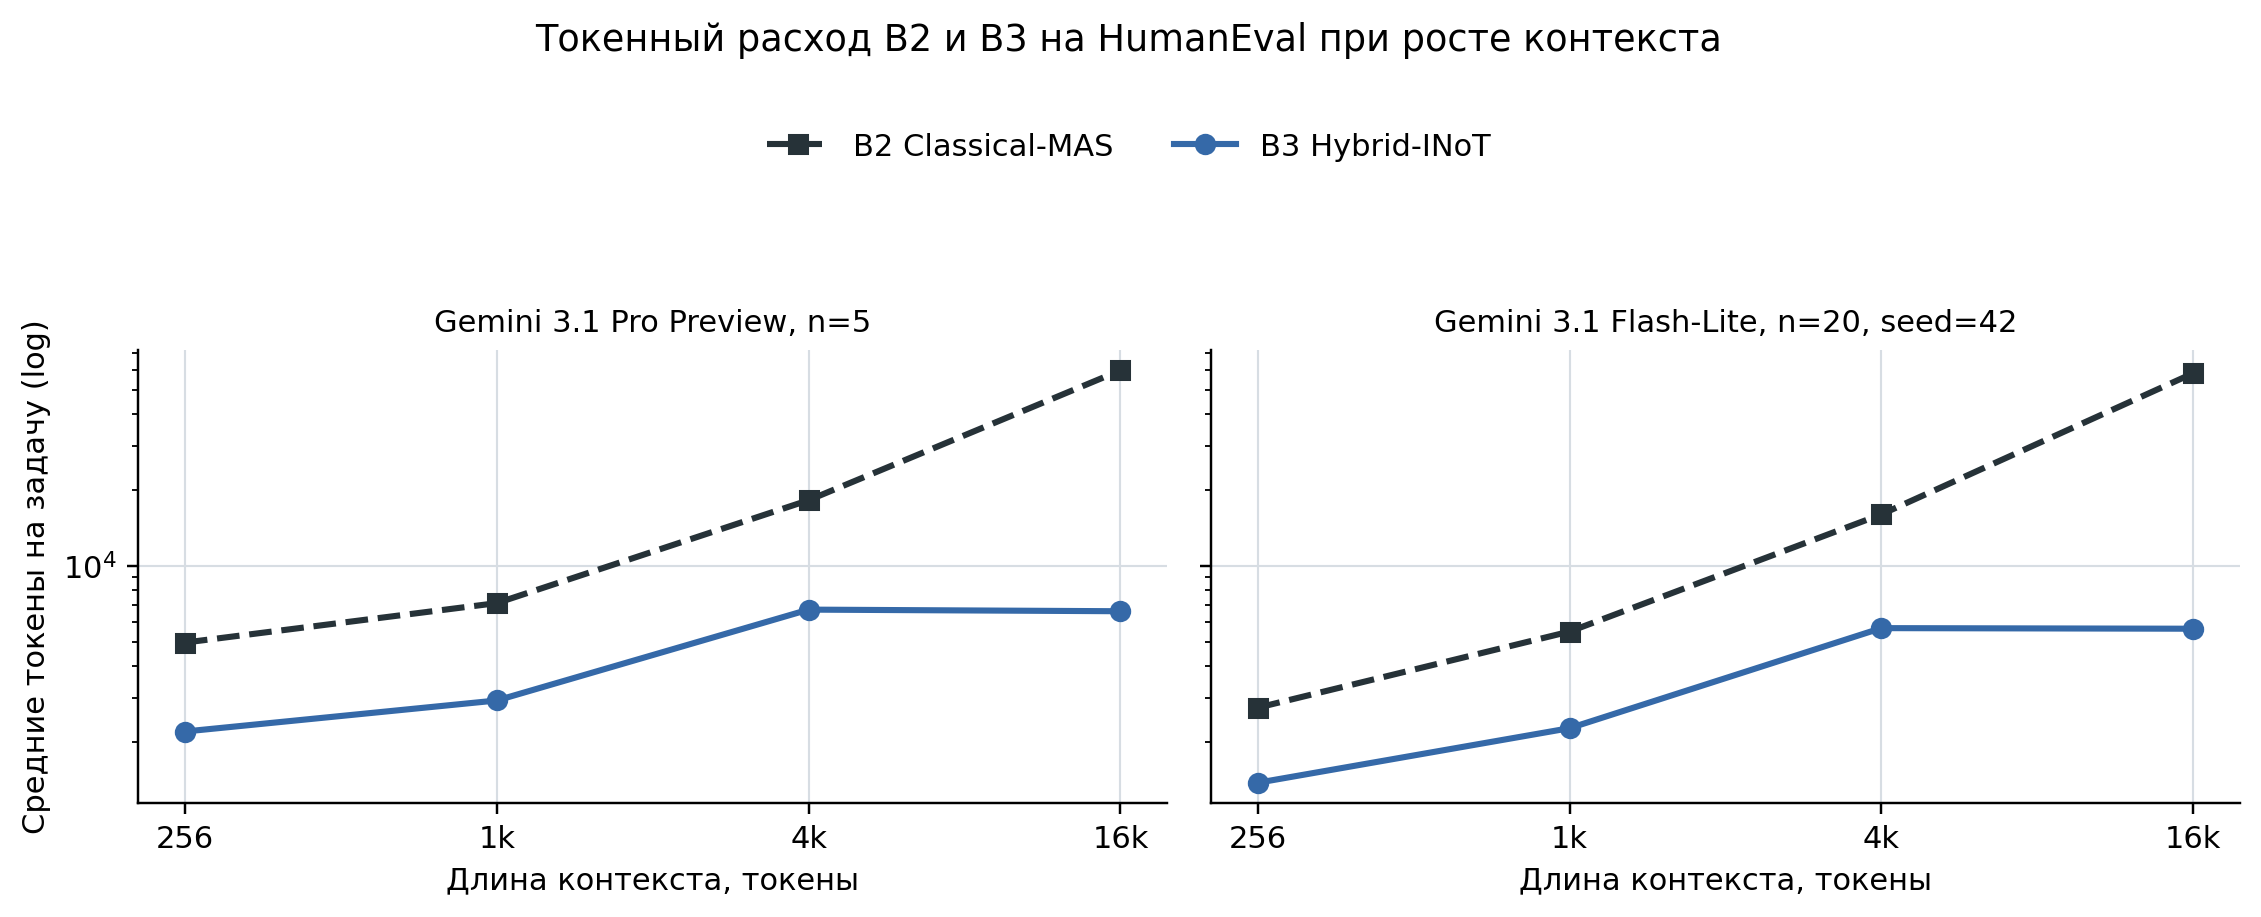
\includegraphics[width=\textwidth]{figures/generated/e3_humaneval_replication.png}
\caption{Средний суммарный токенный расход на задачу. Штриховая линия с квадратами~--- B2 Classical-MAS; сплошная линия с кругами~--- B3 Hybrid-INoT. Ось $y$ логарифмическая. Слева показан сохранённый Pro-пилот ($n=5$ на точку), справа~--- выполненная для статьи репликация Flash-Lite ($n=20$, seed 42).}
\label{fig:e3-replication}
\end{figure}

Покажем вычисление для Pro при 16\,384 целевых токенах:
\[
S_T=100\left(1-\frac{6608.4}{59631.4}\right)=88.9\%,\qquad
S_C=100\left(1-\frac{0.0294908}{0.1407228}\right)=79.0\%.
\]
Поскольку pass@1 обеих конфигураций равен 1, агрегированное отношение средних даёт
\[
U_{B2}=\frac{1}{59631.4}=1.677\cdot10^{-5},\quad
U_{B3}=\frac{1}{6608.4}=1.513\cdot10^{-4},
\]
то есть агрегированное отношение средних даёт рост $U_{\mathrm{tok}}$ 802.4\%. Основной парный estimand сначала вычисляет относительное отношение внутри каждой задачи, а затем усредняет: 805.6\%, task-resampling диапазон устойчивости 756.0--850.4\%.

В Pro-пилоте все парные выигрыши превышают 15\%, но при пяти однонаправленных парах условное одностороннее signed-rank $p=0.03125$ в каждой точке не проходит поправку Холма. В Flash-Lite-прогоне средние по конечному набору внутрипарные приросты равны 106.5\% (task-resampling диапазон 87.5--126.1), 144.8\% (131.9--158.3), 183.3\% (177.3--189.6) и 934.6\% (910.8--959.6). Все 20 пар превышают 15\% в каждой ячейке; условное одностороннее signed-rank $p=9.54\cdot10^{-7}$ проходит поправку Холма. Это вывод о наблюдаемой выборке, а не о среднем популяции.

Для каждой задачи дополнительно оценена четырёхточечная OLS-сводка суммарных токенов по \emph{фактической} длине контекста. Средние значения Flash-Lite равны 3.425 (task-resampling диапазон 3.421--3.430) для B2 и 0.219 (0.216--0.222) для B3 токена на токен контекста; все парные разности положительны (средняя 3.206, диапазон 3.201--3.212; условное signed-rank $p=1.91\cdot10^{-6}$). Для Pro получено 3.410 против 0.234 при условном $p=0.0625$ (рис.~\ref{fig:e3-slope}). Поскольку B3 пересекает границу включения компрессии 4096 токенов, коэффициенты описывают всю сетку и не являются локальными производными; диапазоны также не включают неопределённость seed и повторных API-прогонов.

\begin{figure}[htbp]
\centering
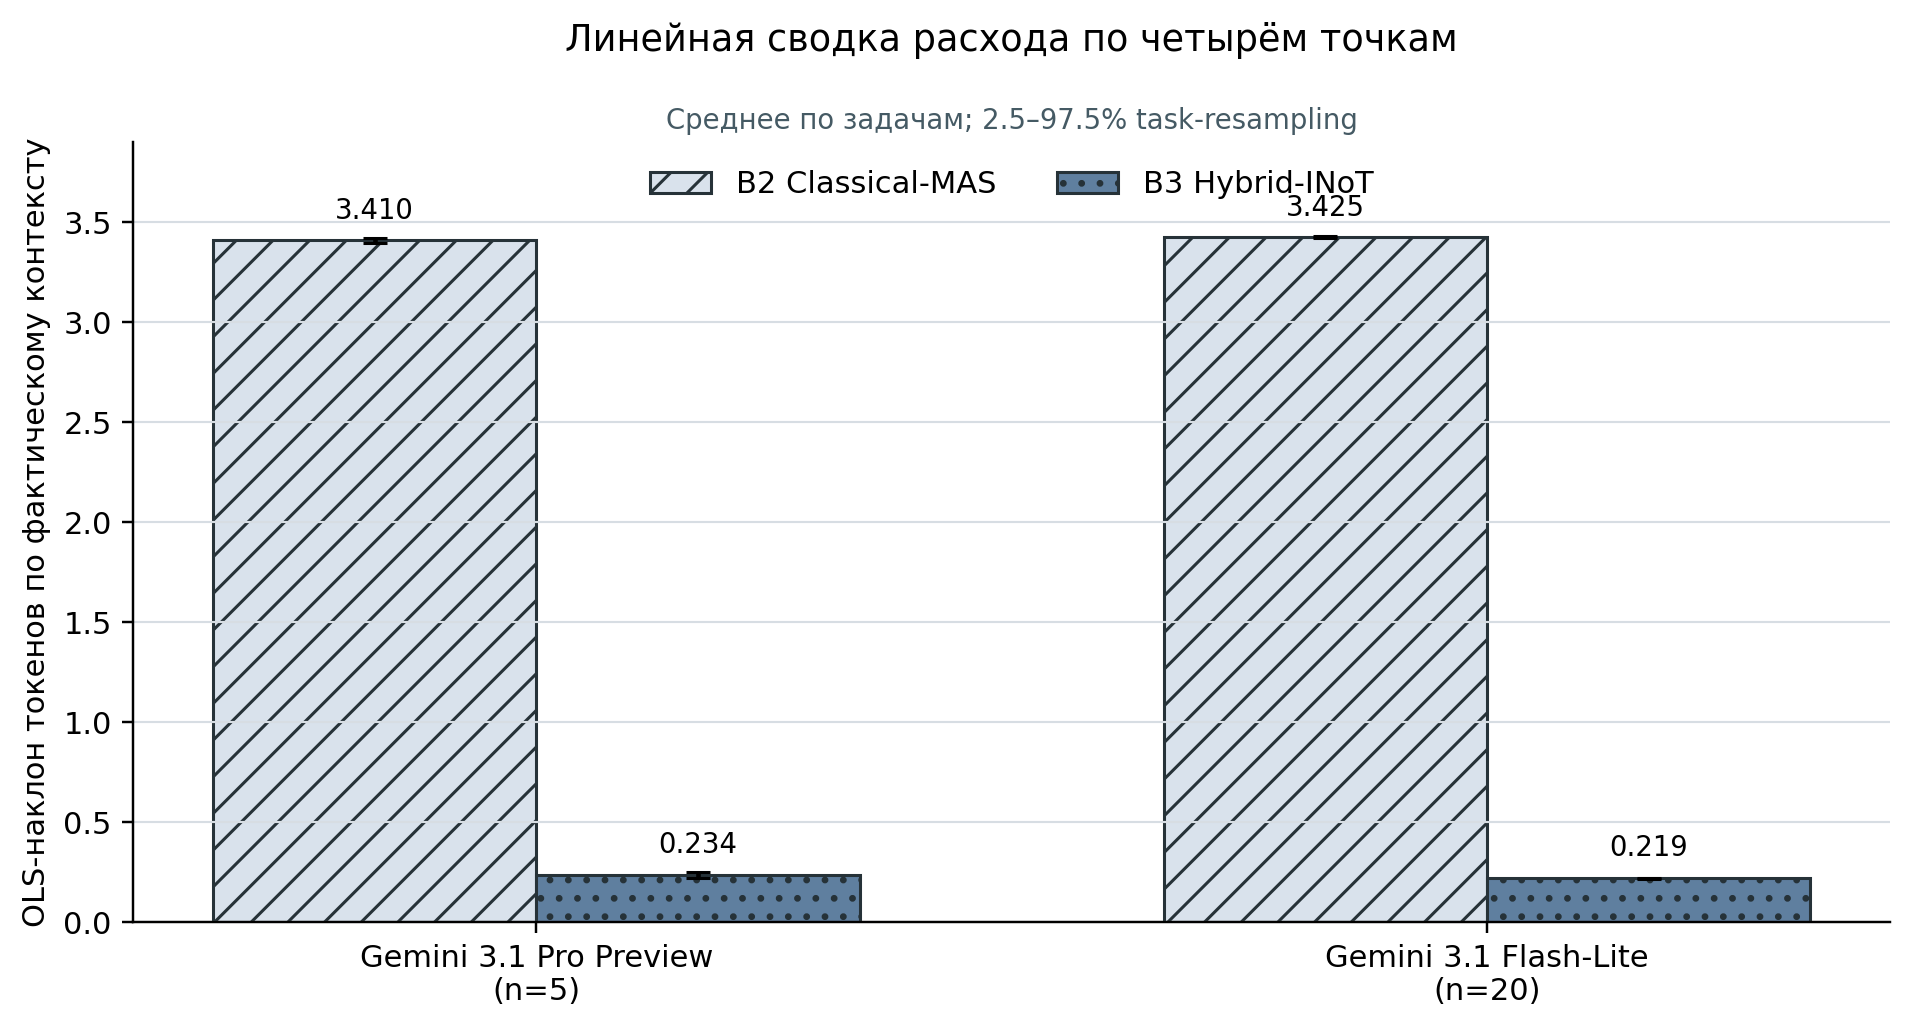
\includegraphics[width=.92\textwidth]{figures/generated/e3_context_scaling_slope.png}
\caption{Task-level четырёхточечные OLS-сводки суммарных токенов по фактической длине контекста. Столбцы~--- средние по задачам, интервалы~--- 2.5--97.5\% task-resampling диапазоны устойчивости. Estimand относится к полным пакетам B2/B3 и не является локальной производной через границу компрессии.}
\label{fig:e3-slope}
\end{figure}

Pass@1${}=1.0$ для обеих архитектур создаёт потолочный эффект. Среди 20 уникальных Flash-Lite-пар вредных исходов нет. В iid-биномиальной модели односторонняя 95\%-я нулевая граница-ориентир равна 13.91~п.п.; чтобы опустить её ниже 2~п.п., требуется не менее 149 пар без вреда, а для всех 164 задач граница составила бы 1.81~п.п. Поскольку взяты первые 20, а не случайная выборка, номинальные уровни служат расчётом мощности, но не гарантией популяционного покрытия. Следовательно, ресурсный подкритерий описательно выполнен в фиксированной выборке, но полная H1 не доказана. E3 не заключает пересечение внутрь сетки: поведение ниже 256 целевых токенов неизвестно, поэтому ни теоретический $\tau^\star$, ни порог маршрутизации не идентифицированы.

\subsection{E2~--- Абляции, критик и параллелизм}\label{subsec:e2}

Абляционный Pro-пилот содержит пять задач. pass@1 равен 1.0 для полной B3 и вариантов без компрессии, критика и самопроверки. Попарные разности агрегированной успешности для B3 против этих трёх вариантов равны $-0.0037$, $-0.0262$ и $0.0000$, с $p=1.0$, $0.5$ и $1.0$; ни одна разность не значима после поправки Холма. Доли токенного расхода компонентов составляют 36.6\% для компрессии, 29.7\% для критика и 33.8\% для самопроверки, но это \emph{накладные расходы}, а не доказанный независимый вклад в качество. На подмножестве ошибок B0 оказалось только две задачи; наблюдаемая доля ошибочных одобрений критика равна нулю, что недостаточно для вывода о надёжности критика.

В E2c среднее время B2 равно 19.28~с, B3~--- 9.76~с; относительное изменение B3 составляет $-49.4\%$, task-resampling диапазон разности B3$-$B2 равен $[-13.05;-6.83]$~с, а условный критерий Вилкоксона при $n=5$ даёт $p=0.0625$. Отдельный детерминированный микротест инструментов действительно показывает, что последовательное выполнение медленнее параллельного на 148.8\%, однако прямое сравнение архитектур не показало ожидаемого проигрыша B3. Поэтому H3 в данном пилоте \emph{не поддержана}; микротест подтверждает лишь механизм, который предстоит изолировать на задачах с реальными независимыми инструментами. В E2d получено семь инверсий ранжирования при вариации весов и $\lambda$; канонически первым оказался вариант без критика. Это указывает на неустойчивость составной метрики и исключает сильный вывод о необходимости каждого компонента.

\subsection{E4~--- Разведочная диагностика согласия малой модели}\label{subsec:e4}

В 20 случаях HumanEval и 20 случаях приближённого SWE-bench Lite Gemini~3.1~Pro Preview генерировал решение, а Flash-Lite выдавал PASS/REJECT. В сохранённом файле есть агрегированные счётчики, но нет решений малой модели по каждому случаю, текстов кандидатов, индивидуальных стоимостей и контрфактических исходов перезапуска. Отклонение неудачного кандидата в этом harness само по себе не предотвращает реализованный повторный вызов. Поэтому исходный policy-estimand из~\eqref{eq:small-model-condition} и H2 невоспроизводим и причинно не оценён; можно сообщить только согласие с сохранённым исходом внешней проверки.

\begin{table}[htbp]
\caption{Агрегированная диагностика screening-процедуры}
\label{tab:e4-results}
\centering
\footnotesize
\begin{tabular}{@{}lrrrrr@{}}
\toprule
Набор & $n$ & Верно/pass & Верно/reject & Ошибка/pass & Ошибка/reject \\
\midrule
HumanEval & 20 & 13 & 0 & 0 & 7 \\
SWE-bench Lite* & 20 & 3 & 2 & 12 & 3 \\
\botrule
\end{tabular}
\end{table}

Для HumanEval согласие равно 1.00 (95\%-й Clopper--Pearson reference-интервал 0.832--1.000), sensitivity, specificity и balanced accuracy также равны 1.00; средняя цена проверки~--- 0.555\% стоимости генерации. Для приближённого SWE-bench согласие 0.30 (reference-интервал 0.119--0.543), sensitivity 0.60, specificity 0.20, balanced accuracy 0.40; цена проверки~--- 0.846\% генерации. Номинальные интервалы предполагают iid-случаи и служат лишь описательными ориентирами фиксированных наборов. Звёздочка существенна: загрузчик не запускает официальный контейнерный SWE-bench harness~\cite{jimenez2023swebench}, а использует извлечение кода и заглушку \texttt{check(\_)}. Эти агрегаты мотивируют будущий интегрированный policy-эксперимент, но не поддерживают H2.

\subsection{E6~--- Межмодельная чувствительность}\label{subsec:e6}

Сохранённый E6 сравнивает Pro и Flash-Lite на контролируемом наборе из десяти случаев для каждой пары архитектура--контекст. Набор содержит повторения трёх семейств функций (\texttt{reverse\_words}, \texttt{count\_peaks}, \texttt{normalize\_path}); pass@1 равен 1.0 во всех ячейках, поэтому эксперимент измеряет стоимость на простом потолочном наборе. При длинах 512, 2048 и 8192 стоимость Flash-Lite составляет 4.8, 6.9 и 9.7\% стоимости Pro для B2 и 4.4, 5.4 и 7.0\% для B3 (рис.~\ref{fig:e6-cost}). Парные различия $U_{\mathrm{tok}}$ значимы ($p=0.001953$; все сравнения проходят поправку Холма), но из-за потолка качества этот результат нельзя обобщать на сложные задачи.

\begin{figure}[htbp]
\centering
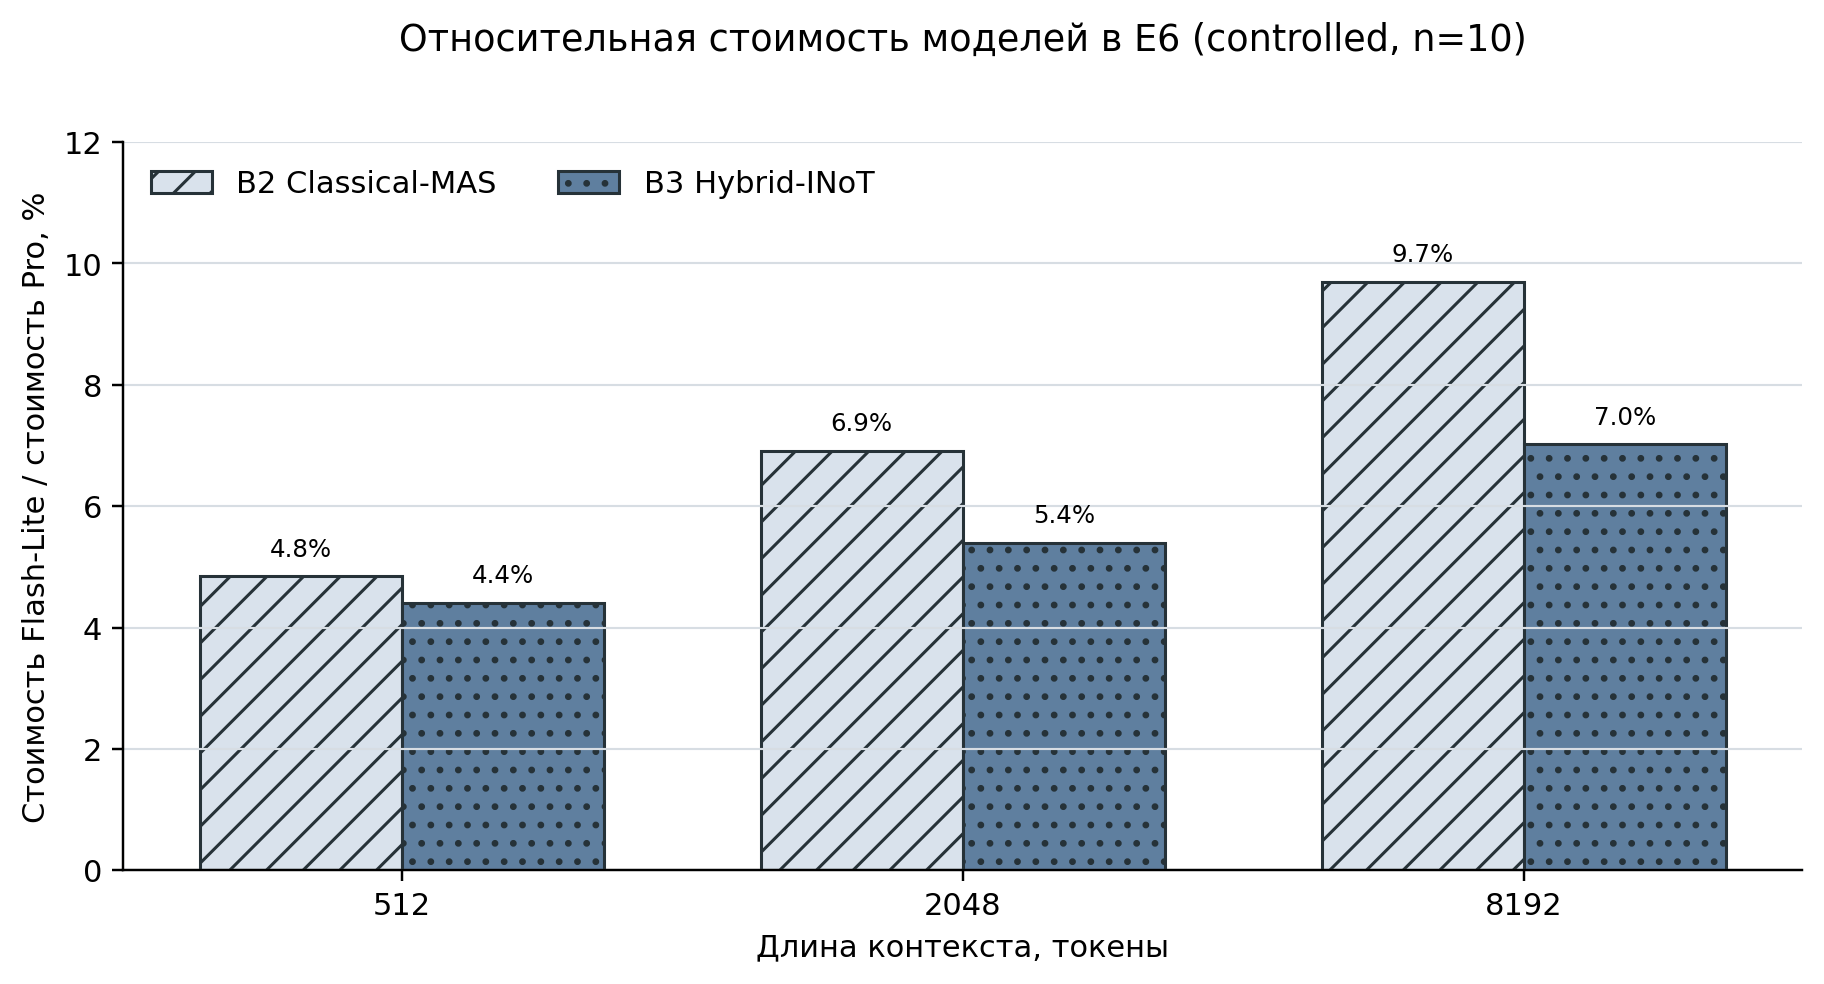
\includegraphics[width=.92\textwidth]{figures/generated/e6_model_cost_ratio.png}
\caption{Отношение средней стоимости Gemini~3.1~Flash-Lite к стоимости Gemini~3.1~Pro Preview в контролируемом E6. Штриховки обеспечивают различимость при чёрно-белой печати.}
\label{fig:e6-cost}
\end{figure}

\subsection{E5~--- Экстраполяция стоимости API-инференса}\label{subsec:e5}

Полный TCO-эксперимент не был завершён: дополнительный запуск был остановлен лимитом провайдера до сохранения \texttt{runs.json} и исключён из анализа. Вместо подмены отсутствующих данных выполнена явно ограниченная аналитическая экстраполяция из двадцати парных Pro-случаев E3 (пять задач на каждую из четырёх длин, равные веса). Для $N$ задач
\begin{equation}
\Delta C_{\mathrm{inf}}(N)=N\cdot
\frac{1}{20}\sum_{i=1}^{20}\left(C_{B2,i}-C_{B3,i}\right).
\label{eq:inference-extrapolation}
\end{equation}
Средняя разность равна \$0.042996 на задачу; при $N=10\,000$ это \$429.96 экономии B3. Поскольку одни и те же пять задач повторяются на четырёх длинах контекста, ресэмплирование пяти \emph{кластеров задач} с сохранением всех четырёх ячеек даёт диапазон устойчивости \$417.33--\$442.90, не имеющий design-based популяционного покрытия. Leave-one-task-out оценки лежат в \$425.20--\$435.51. Среднее сокращение входа и выхода составляет 17\,146.8 и 725.2 токена на случай; все 20 парных разностей положительны. Независимое изменение множителей входной и выходной цены от 0.5 до 1.5 сохраняет положительную экономию во всей сетке (\$214.98--\$644.94; рис.~\ref{fig:e5-sensitivity}).

\begin{figure}[htbp]
\centering
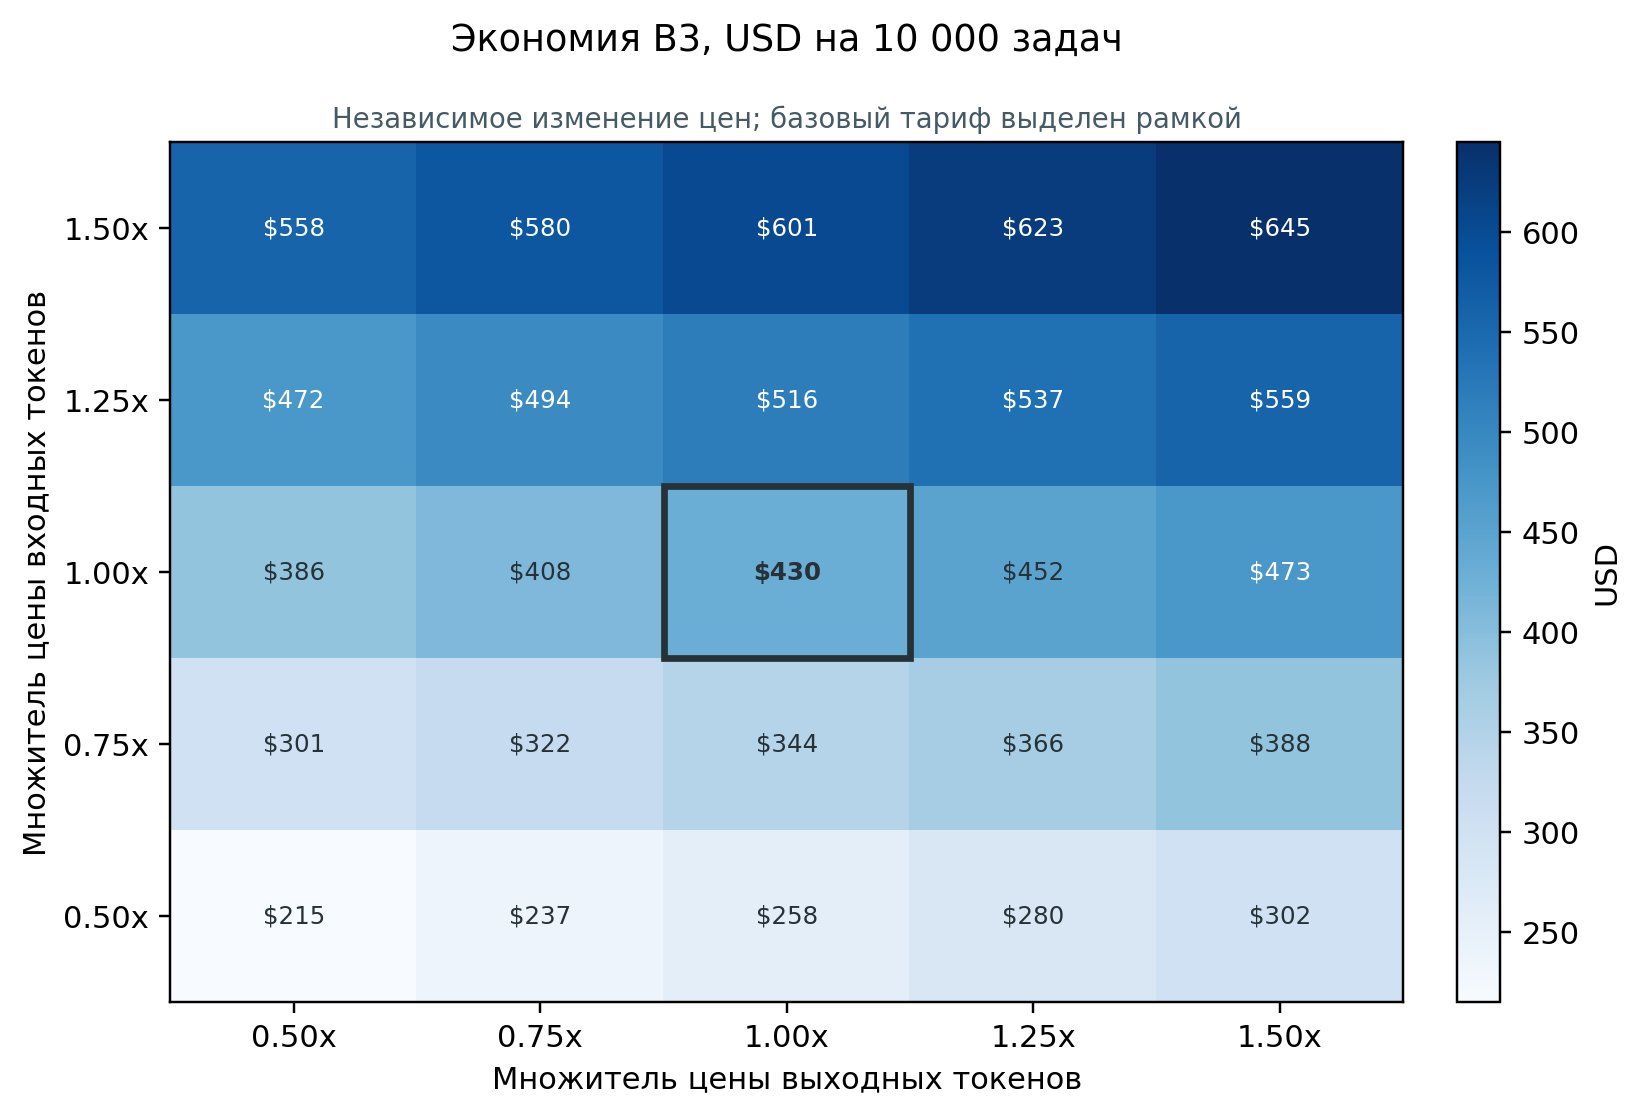
\includegraphics[width=.92\textwidth]{figures/generated/e5_inference_cost_sensitivity.png}
\caption{Экономия API-инференса на 10\,000 задач при независимых множителях входной и выходной цены. Контуром отмечен зафиксированный тариф Pro. Это детерминированная ценовая чувствительность, а не популяционная неопределённость.}
\label{fig:e5-sensitivity}
\end{figure}

\section{Экономическая модель}\label{sec:tco}

\subsection{Граница между инференсом и TCO}

\begin{equation}
\mathrm{TCO}_{\text{month}}=C_{\text{inf}}+C_{\text{hw}}+C_{\text{energy}}+C_{\text{storage}}+C_{\text{ops}}.
\label{eq:tco}
\end{equation}

В работе измерено только $C_{\text{inf}}$ для внешнего API. Аппаратные ресурсы, энергия, хранение, сопровождение, разработка и возможная стоимость задержки не измерялись; следовательно, положительная нижняя граница в E5 доказывает экономию \emph{API-инференса в пилотной смеси}, но не $\Delta\mathrm{TCO}<0$. При использовании управляемого API часть остальных слагаемых включена в цену провайдера непрозрачно, что также не позволяет декомпозировать TCO.

\subsection{Сводный вердикт по гипотезам}

\begin{table}[htbp]
\caption{Соответствие исходных гипотез фактическим данным}
\label{tab:hypothesis-verdict}
\centering
\footnotesize
\begin{tabularx}{\textwidth}{@{}l l X@{}}
\toprule
Гипотеза & Вердикт & Основание \\
\midrule
H1 & в целом не доказана & Каждая Flash-Lite-пара фиксированной выборки превысила ресурсный порог 15\%, но неухудшение качества на 2~п.п. не доказано. \\
H2 & не оценена & E4 сохранил агрегаты screening, но не интегрированную политику перезапуска и не контрфактические стоимости по задачам. \\
H3 & не поддержана & Инструментальный микротест показывает пользу параллелизма, но B3 в прямом пилоте быстрее B2; $n=5$. \\
$\tau^\star$/router & не идентифицированы & Пересечение не заключено в сетке, поведение ниже неё неизвестно, E3 принудительно использует internal B3. \\
\bottomrule
\end{tabularx}
\end{table}

\section{Ограничения и угрозы валидности}\label{sec:limits}

\subsection{Границы интерпретации}

\begin{enumerate}
\item \textbf{Малые и неслучайные выборки.} Использованы первые 5 или 20 задач HumanEval, а не случайная стратифицированная выборка из 164 задач; новый прогон имеет один seed. Это ограничивает статистическую мощность и внешнюю валидность.
\item \textbf{Синтетический контекст.} Длинный вход составлен из других задач HumanEval, а не из истории реального репозитория. Он изолирует цену повторной передачи, но не отражает зависимости и шум промышленной кодовой базы.
\item \textbf{Потолок качества.} В B2/B3 и контролируемом E6 pass@1 равен 1.0. Данные показывают различие расхода, но не дают строгого теста неухудшения качества и не исключают иной результат на сложных задачах.
\item \textbf{Пакетный treatment.} B3 меняет топологию вызовов и, свыше 4096 токенов, отбор контекста. Для атрибуции компонентов нужен факторный дизайн; текущий estimand относится к end-to-end пакету.
\item \textbf{Неполный SWE-bench.} Используемая проверка не является официальным контейнерным протоколом; вывод о решении issue или переносе на реальные репозитории не делается.
\item \textbf{Маршрутизатор не проверен.} E3 всегда вызывает internal B3; точность флагов и контекстный gate не тестировались.
\item \textbf{Post-hoc робастность.} Четырёхточечные OLS-сводки, iid-reference граница вреда и task-cluster диапазон ресэмплирования добавлены после аудита пилота. Это прозрачные диагностики, а не пререгистрированные confirmatory endpoints.
\item \textbf{Аудитируемость E4.} Per-case решения малой модели и контрфактические исходы перезапуска не сохранены, поэтому H2 остаётся неоценённой.
\item \textbf{Дрейф API.} В результатах сохранены имена моделей, параметры, токены, задержка и стоимость, но API-псевдонимы не гарантируют неизменность весов. Неудавшиеся из-за лимита провайдера запуски не включены.
\item \textbf{Ограниченная аудитируемость ответа.} \texttt{runs.json} хранит метрики и usage, но не полный финальный текст решения; независимая постфактум-проверка каждого ответа ограничена.
\item \textbf{Стоимость не равна TCO.} Рисунок~\ref{fig:e5-sensitivity} отражает только API-инференс при заданной смеси контекстов. Остальные слагаемые~\eqref{eq:tco} и производственная нагрузка не измерялись.
\item \textbf{Архитектурные границы.} Истинно независимые подзадачи, необходимость процессной изоляции, ошибки критика и потеря фактов при компрессии могут устранить преимущество B3. Промежуточные ролевые тексты являются вычислительным механизмом, а не достоверным объяснением поведения модели~\cite{turpin2023unfaithful}.
\end{enumerate}

\section{Направления дальнейшего исследования}\label{sec:agenda}

Следующий этап должен устранять выявленные источники неопределённости, а не повторять уже выполненный пилот:
\begin{enumerate}
\item пререгистрировать полный факторный эксперимент $2\times2$: топология вызовов (раздельная/объединённая) $\times$ отбор контекста (выключен/включён);
\item использовать не менее 149 уникальных пар без вредных исходов~--- предпочтительно все 164 HumanEval и несколько seed~--- для точной 2-п.п. цели неухудшения;
\item расширить сетку ниже 256 токенов и включить области выигрыша и проигрыша до оценки crossover или routing gate;
\item сохранять полный вход, выход, хеш промпта, точный идентификатор снимка модели и результат внешнего теста для каждого запуска;
\item заменить приближённый SWE-bench-путь официальным контейнерным harness и провести оценку на случайной выборке репозиториев;
\item повторить E2c на задачах с независимыми реальными инструментами и сопоставить последовательный и параллельный режимы при одинаковой модели;
\item сравнить B3 с Self-Refine, SPP, Self-Collaboration, S2-MAD, Agentless, ReAct и SWE-agent при совпадающих вызовах, контексте и проверке;
\item реализовать E4 как рандомизированный либо парный policy-эксперимент с сохранением каждого решения screening, перезапуска, финального кандидата и стоимости;
\item измерить полный TCO, включая труд сопровождения, задержку, число повторных запусков, инфраструктуру и хранение, на производственном распределении длины контекста.
\end{enumerate}

\section{Заключение}

Hybrid-INoT оценён как интегрированная промежуточная система между внутриконтекстными ролями и внешней мультиагентной оркестрацией. В двух реальных API-пилотах пакет B3 использовал на 49.6--90.3\% меньше токенов, чем сопоставленный B2; четырёхточечная Flash-Lite OLS-сводка равна 3.425 для B2 и 0.219 для B3 токена на токен контекста. Каждая наблюдаемая Flash-Lite-пара превысила ресурсный порог 15\%, а условный rank-based анализ чувствительности прошёл поправку на множественные сравнения, но полная H1 не доказана: 20 потолочных неслучайных пар недостаточно для допуска неухудшения 2 п.п. H2 не оценена агрегированным screening-harness, H3 не поддержана; маршрутизация и атрибуция компонентов остаются открытыми. \$429.96~--- экономия API-инференса для фиксированной смеси, а не популяционный TCO. Защищаемый вывод состоит в том, что полный пакет B3 уменьшает повторную передачу длинного контекста в этих контролируемых наборах; качество, причинный вклад компонентов, польза маршрутизатора и эффект на реальных репозиториях требуют мощного пререгистрированного исследования.

\backmatter
\selectlanguage{russian}

\section*{Доступность данных и кода}
Код исследования, конфигурации и исходные результаты доступны в неизменяемом commit, указанном в~\cite{inotresearch2026}. Репозиторий статьи содержит входы репликации Flash-Lite, SHA-256 manifest, переносимый evidence snapshot и скрипт построения рисунков. Скрипт пересчитывает из строк E3 агрегаты, парные диагностики, контекстные сводки, агрегированную E4 screening-таблицу и E5-экстраполяцию; готовые E2/E6-сводки импортируются с хешами, а не пересчитываются. Полные сгенерированные ответы в сохранённом \texttt{runs.json} отсутствуют, поэтому pass/fail labels и исходные внешние тесты нельзя независимо воспроизвести только из артефакта статьи. Эти границы и хеш аналитического скрипта записаны в evidence snapshot.

\section*{Декларации}
\textbf{Финансирование:} внешнее финансирование не заявлено. \textbf{Конфликт интересов:} автор заявляет об отсутствии конфликта интересов. \textbf{Этика:} использованы публичные программные бенчмарки; люди и персональные данные в исследовании не участвуют. \textbf{Вклад автора:} Д.П. спроектировал исследование, реализовал системы, провёл эксперименты, аудировал свидетельства и подготовил рукопись.

\selectlanguage{english}

\begin{thebibliography}{99}

\bibitem{sun2025inot}
H.~Sun and S.~Zeng, ``Introspection of Thought Helps AI Agents,'' arXiv preprint arXiv:2507.08664, 2025.

\bibitem{ko2007}
A.~J.~Ko, R.~DeLine, and G.~Venolia, ``Information Needs in Collocated Software Development Teams,'' in \emph{Proc.\ 29th Int.\ Conf.\ Software Engineering}, 2007, pp.~344--353.

\bibitem{parnin2011}
C.~Parnin and S.~Rugaber, ``Resumption Strategies for Interrupted Programming Tasks,'' \emph{Software Quality Journal}, vol.~19, no.~1, pp.~5--34, 2011.

\bibitem{goncalves2011}
M.~K.~Goncalves, C.~R.~B.~de Souza, and V.~M.~Gonzalez, ``Collaboration, Information Seeking and Communication,'' \emph{J.\ Universal Computer Science}, vol.~17, no.~11, pp.~1529--1550, 2011.

\bibitem{wei2022cot}
J.~Wei \emph{et al.}, ``Chain-of-Thought Prompting Elicits Reasoning in Large Language Models,'' in \emph{NeurIPS}, vol.~35, 2022, pp.~24824--24837.

\bibitem{yao2022react}
S.~Yao \emph{et al.}, ``ReAct: Synergizing Reasoning and Acting in Language Models,'' \emph{ICLR}, 2023.

\bibitem{madaan2023selfrefine}
A.~Madaan \emph{et al.}, ``Self-Refine: Iterative Refinement with Self-Feedback,'' \emph{NeurIPS}, 2023.

\bibitem{shinn2023reflexion}
N.~Shinn \emph{et al.}, ``Reflexion: Language Agents with Verbal Reinforcement Learning,'' \emph{NeurIPS}, 2023.

\bibitem{wang2024spp}
Z.~Wang \emph{et al.}, ``Unleashing Cognitive Synergy in Large Language Models: A Task-Solving Agent through Multi-Persona Self-Collaboration,'' in \emph{Proc.\ NAACL-HLT}, 2024, pp.~257--279, doi:10.18653/v1/2024.naacl-long.15.

\bibitem{dong2024selfcollaboration}
Y.~Dong, X.~Jiang, Z.~Jin, and G.~Li, ``Self-Collaboration Code Generation via ChatGPT,'' \emph{ACM Trans.\ Software Engineering and Methodology}, vol.~33, no.~7, art.~189, pp.~1--38, 2024, doi:10.1145/3672459.

\bibitem{zeng2025s2mad}
Z.~Zeng \emph{et al.}, ``S2-MAD: Breaking the Token Barrier to Enhance Multi-Agent Debate Efficiency,'' in \emph{Proc.\ NAACL-HLT}, 2025, pp.~9393--9408, doi:10.18653/v1/2025.naacl-long.475.

\bibitem{xia2024agentless}
C.~S.~Xia, Y.~Deng, S.~Dunn, and L.~Zhang, ``Agentless: Demystifying LLM-based Software Engineering Agents,'' arXiv:2407.01489, 2024.

\bibitem{turpin2023unfaithful}
M.~Turpin, J.~Michael, E.~Perez, and S.~R.~Bowman, ``Language Models Don't Always Say What They Think: Unfaithful Explanations in Chain-of-Thought Prompting,'' \emph{NeurIPS}, 2023.

\bibitem{weiss1999}
G.~Weiss, \emph{Multiagent Systems}. MIT Press, 1999.

\bibitem{wooldridge2009}
M.~Wooldridge, \emph{An Introduction to MultiAgent Systems}, 2nd~ed. Wiley, 2009.

\bibitem{hong2023metagpt}
S.~Hong \emph{et al.}, ``MetaGPT: Meta Programming for A Multi-Agent Collaborative Framework,'' \emph{ICLR}, 2024.

\bibitem{qian2023chatdev}
C.~Qian \emph{et al.}, ``ChatDev: Communicative Agents for Software Development,'' \emph{ACL}, 2024.

\bibitem{guo2024survey}
T.~Guo \emph{et al.}, ``Large Language Model based Multi-Agents: A Survey of Progress and Challenges,'' arXiv:2402.01680, 2024.

\bibitem{qian2024scaling}
C.~Qian \emph{et al.}, ``Scaling Large Language Model-based Multi-Agent Collaboration,'' arXiv:2406.07155, 2024.

\bibitem{jimenez2023swebench}
C.~E.~Jimenez \emph{et al.}, ``SWE-bench: Can Language Models Resolve Real-World GitHub Issues?,'' \emph{ICLR}, 2024.

\bibitem{yang2024sweagent}
J.~Yang \emph{et al.}, ``SWE-agent: Agent-Computer Interfaces Enable Automated Software Engineering,'' \emph{NeurIPS}, 2024.

\bibitem{chen2021humaneval}
M.~Chen \emph{et al.}, ``Evaluating Large Language Models Trained on Code,'' arXiv:2107.03374, 2021.

\bibitem{austin2021mbpp}
J.~Austin \emph{et al.}, ``Program Synthesis with Large Language Models,'' arXiv:2108.07732, 2021.

\bibitem{jiang2023longllmlingua}
H.~Jiang \emph{et al.}, ``LongLLMLingua: Accelerating and Enhancing LLMs in Long Context Scenarios via Prompt Compression,'' \emph{ACL}, 2024.

\bibitem{pan2024llmlingua2}
Z.~Pan \emph{et al.}, ``LLMLingua-2: Data Distillation for Efficient and Faithful Task-Agnostic Prompt Compression,'' \emph{ACL Findings}, 2024.

\bibitem{jia2026compression}
H.~Jia, E.~T.~Barr, and S.~Mechtaev, ``Compressing Code Context for LLM-based Issue Resolution,'' arXiv:2603.28119, 2026.

\bibitem{bi2024cocogen}
Z.~Bi \emph{et al.}, ``Iterative Refinement of Project-Level Code Context for Precise Code Generation with Compiler Feedback,'' arXiv:2403.16792, 2024.

\bibitem{su2025static}
C.-Y.~Su and C.~McMillan, ``Do Code LLMs Do Static Analysis?,'' arXiv:2505.12118, 2025.

\bibitem{sepidband2025complexity}
M.~Sepidband, H.~Taherkhani, S.~Wang, and H.~Hemmati, ``Enhancing LLM-Based Code Generation with Complexity Metrics,'' arXiv:2505.23953, 2025.

\bibitem{iso25010}
ISO/IEC 25010:2023, ``Systems and software engineering~--- SQuaRE~--- Product quality model,'' ISO, 2023.

\bibitem{mccabe1976}
T.~J.~McCabe, ``A Complexity Measure,'' \emph{IEEE Trans.\ Software Engineering}, vol.~SE-2, no.~4, pp.~308--320, 1976.

\bibitem{wilcoxon1945}
F.~Wilcoxon, ``Individual Comparisons by Ranking Methods,'' \emph{Biometrics Bulletin}, vol.~1, no.~6, pp.~80--83, 1945.

\bibitem{holm1979}
S.~Holm, ``A Simple Sequentially Rejective Multiple Test Procedure,'' \emph{Scandinavian J.\ Statistics}, vol.~6, no.~2, pp.~65--70, 1979.

\bibitem{inotresearch2026}
D.~Privezentsev, ``INoT\_Research: reproducible experiments for Hybrid-INoT,'' GitHub repository, commit \texttt{010211ee5775185e8330ab6cde06e912c2adcb9e}, 2026. [Online]. Available: \url{https://github.com/daniil-novel/INoT_Research}. Accessed: 28 July 2026.

\bibitem{openrouterpro2026}
OpenRouter, ``Gemini 3.1 Pro Preview~--- pricing,'' 2026. [Online]. Available: \url{https://openrouter.ai/google/gemini-3.1-pro-preview/pricing}. Accessed: 26 July 2026.

\bibitem{openrouterflash2026}
OpenRouter, ``Gemini 3.1 Flash Lite Preview~--- pricing,'' 2026. [Online]. Available: \url{https://openrouter.ai/google/gemini-3.1-flash-lite/pricing}. Accessed: 26 July 2026.

\end{thebibliography}

\end{document}
